\documentclass[12pt, a4paper, oneside]{report}

% Encoding and language
\usepackage[utf8]{inputenc}
\usepackage[T1]{fontenc}
\usepackage[english]{babel}

% Times New Roman font
\usepackage{mathptmx}

% Margins per FSEGA guide (2.54cm on all sides)
\usepackage[top=2.54cm, bottom=2.54cm, left=2.54cm, right=2.54cm]{geometry}

% 1.5 line spacing
\usepackage{setspace}
\onehalfspacing

% Graphics and plots
\usepackage{pgfplots}
\pgfplotsset{compat=1.18}
\usepackage{graphicx}
\usepackage{float}
\usepackage{subcaption}

% Tables
\usepackage{booktabs}
\usepackage{multirow}
\usepackage{array}
\usepackage{longtable}
\usepackage{tabularx}

% Math
\usepackage{amsmath}
\usepackage{amssymb}

% Code listings
\usepackage{listings}
\lstset{
    basicstyle=\ttfamily\small,
    breaklines=true,
    frame=single,
    numbers=left,
    numberstyle=\tiny,
    tabsize=2
}

% Tikz for topology diagrams
\usepackage{tikz}
\usetikzlibrary{positioning, calc}

% Hyperlinks
\usepackage[hidelinks]{hyperref}

% Bibliography (author-year format per FSEGA guide)
\usepackage[authoryear,round]{natbib}
\bibpunct{(}{)}{;}{a}{,}{,}

% Captions
\usepackage{caption}
\captionsetup{font=small, labelfont=bf}

% Custom colors for plots
\definecolor{starcolor}{HTML}{0033CC}
\definecolor{ringcolor}{HTML}{F59E0B}
\definecolor{meshcolor}{HTML}{09090B}
\definecolor{treecolor}{HTML}{10B981}
\definecolor{buscolor}{HTML}{EF4444}

% Chapter formatting per FSEGA guide
\usepackage{titlesec}
\titleformat{\chapter}[display]
    {\normalfont\fontsize{14}{16}\bfseries}
    {\MakeUppercase{\chaptertitlename}\ \thechapter}{12pt}
    {\fontsize{14}{16}\bfseries}
\titleformat{name=\chapter,numberless}[display]
    {\normalfont\fontsize{14}{16}\bfseries}
    {}{0pt}
    {\fontsize{14}{16}\bfseries}
\titlespacing*{\chapter}{0pt}{12pt}{12pt}
\titlespacing*{name=\chapter,numberless}{0pt}{12pt}{12pt}
\titleformat{\section}
    {\normalfont\fontsize{13}{15}\bfseries}
    {\thesection}{1em}{}
\titlespacing*{\section}{0pt}{12pt}{12pt}
\titleformat{\subsection}
    {\normalfont\fontsize{12}{14}\itshape\centering}
    {\thesubsection}{1em}{}
\titlespacing*{\subsection}{0pt}{12pt}{12pt}

% Paragraph spacing per FSEGA guide (1cm first-line indent, no extra
% spacing between paragraphs; LaTeX already suppresses the indent on the
% paragraph immediately following a chapter/section heading)
\setlength{\parindent}{1cm}
\setlength{\parskip}{0pt}

% pgfplots bar chart style
\pgfplotsset{
    topology bar/.style={
        ybar,
        bar width=10pt,
        enlarge x limits=0.15,
        ylabel style={font=\small},
        xlabel style={font=\small},
        tick label style={font=\footnotesize},
        legend style={font=\footnotesize, at={(0.5,-0.25)}, anchor=north, legend columns=-1},
        nodes near coords,
        nodes near coords style={font=\tiny},
        every node near coord/.append style={rotate=90, anchor=west},
        width=0.95\textwidth,
        height=7cm,
    },
    topology line/.style={
        width=0.95\textwidth,
        height=7cm,
        ylabel style={font=\small},
        xlabel style={font=\small},
        tick label style={font=\footnotesize},
        legend style={font=\footnotesize, at={(0.5,-0.25)}, anchor=north, legend columns=-1},
        grid=major,
        grid style={dashed, gray!30},
        mark size=2pt,
    }
}

\begin{document}

% Title page
\begin{titlepage}
    \centering
    \vspace*{1cm}

    {\large BABE\c{S}-BOLYAI UNIVERSITY}\\[0.3cm]
    {\large FACULTY OF ECONOMICS AND BUSINESS ADMINISTRATION}\\[0.3cm]
    {\large Cluj-Napoca}\\[0.5cm]
    {\large Master's Programme: Business Modelling and Distributed Computing}

    \vspace{3cm}

    {\Large \textbf{MASTER'S THESIS}}

    \vspace{1.5cm}

    {\LARGE \textbf{THE INFLUENCE OF NETWORK TOPOLOGIES ON THE RAFT CONSENSUS ALGORITHM: A SIMULATION-BASED ANALYSIS}}

    \vspace{3cm}

    \begin{minipage}{0.45\textwidth}
        \begin{flushleft}
            \textbf{Scientific supervisor:}\\
            Lect.~univ.~dr.~Stan Alexandru
        \end{flushleft}
    \end{minipage}
    \hfill
    \begin{minipage}{0.45\textwidth}
        \begin{flushright}
            \textbf{Student:}\\
            Socaci Marius-Cristian
        \end{flushright}
    \end{minipage}

    \vfill
    {\large 2026}
\end{titlepage}

% Table of Contents
\pagenumbering{roman}

% Abstract
\chapter*{Abstract}
\addcontentsline{toc}{chapter}{Abstract}

\noindent This thesis investigates how network topology shapes the behaviour of the Raft consensus algorithm, addressing a gap in the literature, which typically assumes a fully connected or abstracted network. We built a discrete-event simulation framework in Python implementing the core Raft state machine within five canonical topologies (Star, Ring, Mesh, Tree, Bus), with shortest-path routing, configurable delay and packet loss, node failures and recoveries, and reproducible seeded runs, accessible via a React/FastAPI web dashboard. Seven experimental campaigns examined baseline performance, scalability, sensitivity to delay and packet loss, fault tolerance, leader-failure recovery, and combined stress, each repeated five to ten times. Results reveal a consistent ordering: Mesh achieves the lowest latency, most predictable elections and strongest resilience to packet loss; Star and Tree degrade abruptly once faults strike their critical nodes; Ring and Bus scale poorly as path length grows, and under combined stress only Mesh sustains the target throughput.

\textbf{Keywords:} Raft, consensus, distributed systems, network topology, simulation, fault tolerance, leader election, replicated state machine, performance evaluation.

\newpage

\tableofcontents
\newpage

% List of Tables
\listoftables
\newpage

% List of Figures
\listoffigures
\newpage

% List of Abbreviations
\chapter*{List of Abbreviations}
\addcontentsline{toc}{chapter}{List of Abbreviations}

\begin{tabular}{ll}
API & Application Programming Interface \\
JSON & JavaScript Object Notation \\
LAN & Local Area Network \\
REST & Representational State Transfer \\
RPC & Remote Procedure Call \\
\end{tabular}

\newpage

% Start main content
\pagenumbering{arabic}
\setcounter{page}{1}

\chapter{Introduction}
\label{ch:introduction}

Distributed systems form the backbone of modern computing infrastructure. From cloud platforms serving billions of users to financial trading systems processing millions of transactions per second, these systems depend on the ability of multiple independent nodes to coordinate and agree on a shared state. The mechanism that enables this coordination is known as consensus, and it remains one of the most studied problems in distributed computing.

The Raft consensus algorithm, proposed by \citet{ongaro2014}, was designed as a more understandable alternative to Paxos \citep{lamport1998}. Since its publication, Raft has seen widespread adoption in production systems including etcd \citep{etcd2024}, CockroachDB \citep{cockroachdb2024}, and HashiCorp Consul \citep{consul2024}. Its decomposition into leader election, log replication, and safety makes it both practical to implement and amenable to formal analysis.

While the correctness properties of Raft have been extensively studied, its performance characteristics under varying network conditions have received less systematic treatment. In particular, the relationship between the underlying network topology and the algorithm's behaviour presents an open area for investigation. Real-world deployments rarely operate on fully connected networks. Data centres use hierarchical tree-like structures. Wide-area networks may impose star or ring configurations. Edge computing environments may rely on bus-like topologies. Each of these imposes different constraints on message latency, path redundancy, and fault tolerance.

\section{Motivation}

The motivation for this work is twofold. First, existing literature on Raft performance tends to assume either a fully connected network or abstract away the network layer entirely. This leaves a gap in understanding how realistic network constraints affect consensus behaviour. Second, practitioners deploying Raft-based systems must make infrastructure decisions about network design, and currently lack quantitative guidance on how topology choice impacts consensus performance.

Consider a distributed database deployed across five data centres. If the network connecting these centres follows a star topology with a central hub, the failure of that hub partitions the entire cluster. If it follows a mesh topology, any single link failure leaves all nodes reachable through alternative paths. These architectural differences directly affect leader election times, message overhead, and the system's ability to maintain consensus under failures.

\section{Research Objectives}

This thesis investigates the following research questions:

\begin{enumerate}
    \item How does network topology affect leader election time in the Raft consensus algorithm?
    \item What is the relationship between topology structure and message overhead during steady-state operation?
    \item How do different topologies respond to node failures and network degradation?
    \item Which topologies provide the best trade-offs between performance and fault tolerance under realistic conditions?
\end{enumerate}

To answer these questions, we developed a discrete-event simulation framework that implements the core Raft protocol and models five common network topologies: Star, Ring, Mesh (fully connected), Tree (binary hierarchy), and Bus (linear chain). We conducted seven experimental campaigns covering baseline performance, scalability with cluster size, sensitivity to message delay and packet loss, fault tolerance behaviour, leader failure recovery, and combined stress conditions.

\section{Methodology Overview}

Our approach is simulation-based. We implemented a tick-driven simulation engine in Python that models the Raft state machine for each node, computes shortest-path routing through the topology graph, and applies configurable message delays and packet loss per hop. Each experiment was repeated multiple times with different random seeds to obtain statistically meaningful results.

The simulation captures the following metrics at each run: leader election time, total messages sent, average message latency (in both hops and ticks), convergence time, message drop rate, log replication throughput, and election count. These metrics are aggregated across runs using standard statistical measures (mean, standard deviation, minimum, maximum).

\section{Thesis Structure}

The remainder of this thesis is organised as follows.

Chapter~\ref{ch:background} presents the theoretical background, covering distributed consensus, the Raft algorithm, and network topology theory. Chapter~\ref{ch:methodology} describes the simulation framework, its architecture, and implementation details. Chapter~\ref{ch:experiments} defines the experimental setup, including scenarios, parameters, and metrics. Chapter~\ref{ch:results} presents the experimental results with quantitative analysis. Chapter~\ref{ch:discussion} interprets the findings, discusses their implications, and acknowledges limitations. Chapter~\ref{ch:conclusions} summarises the contributions and suggests directions for future work.


\chapter{Theoretical Background}
\label{ch:background}

This chapter lays the conceptual groundwork for the rest of the thesis. It opens by asking why distributed systems need a consensus mechanism at all, then works through the Raft algorithm step by step, with particular emphasis on leader election, log replication and the invariants that make the algorithm safe. The final part of the chapter turns to network topology theory, introducing the structural metrics that will later be used to compare how messages propagate across the five topologies under study.

\section{Distributed Systems and the Need for Consensus}

Following \citet{tanenbaum2017} and \citet{coulouris2011}, we take a distributed system to be a set of autonomous computers, each with its own memory, clock and failure mode, that cooperate closely enough that a user experiences them as a single machine. It is precisely this requirement -- many independent parts behaving as one -- that makes distributed systems simultaneously powerful and difficult to engineer.

Among the properties such a system must provide, consistency is usually the most important: once a client has written a value, it expects any later read to return that value, no matter which replica answers the request. Providing this guarantee is hard because the network linking the replicas may lose, delay or reorder messages, and because any replica can crash at any moment. Funnelling every request through a single designated node would sidestep the problem, but it would simply move the single point of failure onto that node. The standard alternative is to keep several copies of the state and run a consensus protocol that keeps every replica's view of the operation sequence in agreement.

Formally, consensus asks $n$ processes, each proposing a value, to agree on exactly one of those values, even though as many as $f$ of the processes may fail. \citet{lamport1998} characterises a correct consensus algorithm by four properties:

\begin{itemize}
    \item \textbf{Validity:} If every correct process proposes the same value, that value must be the one decided.
    \item \textbf{Agreement:} No two correct processes decide on different values.
    \item \textbf{Termination:} Every correct process eventually reaches a decision.
    \item \textbf{Integrity:} A process decides at most once.
\end{itemize}

A well-known impossibility result due to \citet{flp1985} shows that no deterministic algorithm running in a purely asynchronous system -- one where message delays are unbounded -- can guarantee all four properties if even a single process might fail. Practical algorithms work around this by abandoning pure asynchrony: they rely on timeouts to guess that a process has failed, and they assume the system is \emph{eventually synchronous}, meaning that message delays are bounded for long enough, often enough, that the algorithm can keep making progress.

\section{From Paxos to Raft}

Paxos held the position of default consensus algorithm for nearly two decades. \citet{lamport1998} introduced it, and the more accessible follow-up \citep{lamport2001} cemented its role as the theoretical basis for state-machine replication \citep{schneider1990}. Yet for all its elegance, Paxos has a long-standing reputation for being hard to follow and harder still to implement without subtle errors; systems that advertise Paxos compliance frequently diverge from the original specification in ways that introduce exactly such errors.

Raft, introduced by \citet{ongaro2014}, was a direct response to this state of affairs: ease of comprehension was treated as a design goal in its own right rather than an afterthought. Instead of presenting consensus as a single monolithic protocol, the authors split it into three pieces -- choosing a leader, replicating the log, and guaranteeing safety -- each of which can largely be studied on its own. Combined with clean interfaces between these pieces and a deliberate avoidance of optional optimisations, this structure is, by the authors' own user studies, considerably easier for newcomers to grasp than Paxos. The approach has proved popular in practice: Raft now underpins etcd \citep{etcd2024} (the configuration store behind Kubernetes), CockroachDB, HashiCorp Consul, TiKV and a range of other systems.

\section{The Raft Algorithm}

At the heart of Raft is a log that every server keeps a copy of. Each entry in this log encodes a command destined for the local state machine, and the algorithm's central job is to keep these copies in step: as long as every server applies the same commands in the same order, their state machines remain identical.

\subsection{Server States}

At any given moment, a Raft server occupies exactly one of three roles.

\begin{itemize}
    \item \textbf{Leader:} the sole server authorised to handle client requests; it replicates log entries to the rest of the cluster and keeps followers informed via periodic heartbeats.
    \item \textbf{Follower:} a passive role that only responds to RPCs initiated by a leader or a candidate, and never originates communication itself.
    \item \textbf{Candidate:} a temporary role adopted while a new leader is being chosen.
\end{itemize}

Every server begins life as a follower. If a follower hears nothing from a leader before its randomised election timeout elapses, it promotes itself to candidate and triggers an election.

\begin{figure}[H]
\centering
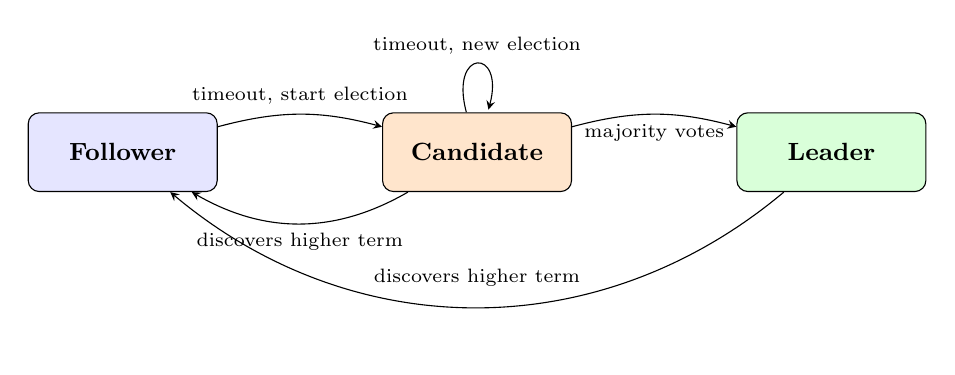
\begin{tikzpicture}[scale=1.0,
    state/.style={rectangle, draw, rounded corners, minimum width=2.4cm, minimum height=1cm, font=\small\bfseries, align=center},
    every edge/.style={draw, ->, >=stealth, font=\scriptsize}]
\node[state, fill=blue!10] (f) at (0,0) {Follower};
\node[state, fill=orange!20] (c) at (4.5,0) {Candidate};
\node[state, fill=green!15] (l) at (9,0) {Leader};

\draw[->, >=stealth] (f) edge[bend left=15] node[above, font=\scriptsize] {timeout, start election} (c);
\draw[->, >=stealth] (c) edge[bend left=15] node[below, font=\scriptsize] {majority votes} (l);
\draw[->, >=stealth] (c) edge[bend left=30] node[below, font=\scriptsize] {discovers higher term} (f);
\draw[->, >=stealth] (l) edge[bend left=40] node[above=4pt, font=\scriptsize] {discovers higher term} (f);
\draw[->, >=stealth] (c) edge[loop above] node[font=\scriptsize] {timeout, new election} (c);
\end{tikzpicture}
\caption{The three states of a Raft server and the transitions between them.}
\label{fig:raft_states}
\end{figure}

\subsection{Terms}

Time in Raft is partitioned into consecutively numbered \emph{terms} with no fixed duration. Every term opens with an attempt to elect a leader. When that attempt succeeds, the elected server governs the cluster until the term ends; when it fails -- typically because the vote was split between several candidates -- a new term begins immediately and the process repeats. Because every RPC is tagged with the sender's term number, terms double as a logical clock: any server that observes a term higher than its own immediately steps down to follower (if it was not one already) and adopts the higher term, allowing the cluster to discard stale leaders and outdated information without relying on synchronised clocks.

\subsection{Leader Election}

An election begins when a follower's timer runs out: the server switches to candidate, increments its term counter, casts a vote for itself, and sends a \texttt{RequestVote} RPC to every peer. Whichever candidate first gathers votes from a majority of the cluster becomes the new leader. Each server, however, votes for only the first candidate it encounters in a given term, and only if that candidate's log is at least as current as its own -- a rule known as the \emph{election restriction}. This restriction is what ensures that no entry already committed can ever be lost when leadership changes hands.

Should the vote split between competing candidates, the term ends without a leader and a fresh election follows. To keep such splits rare, and to guarantee that the cluster keeps making progress, Raft draws each server's election timeout from a random distribution -- commonly uniform between 150 and 300 milliseconds in production deployments.

\subsection{Log Replication}

After winning an election, a leader begins servicing client requests: each request becomes a new entry appended to the leader's log, which is then propagated to every follower via an \texttt{AppendEntries} RPC. Once a majority of servers have acknowledged storing the entry, it is considered \emph{committed}; the leader applies it to its own state machine and reports the result back to the client.

An \texttt{AppendEntries} RPC may carry any number of entries, including none at all -- an empty RPC serves purely as a heartbeat, and receiving one is enough for a follower to restart its election timer, so a healthy leader never triggers a needless election. To keep logs consistent across the cluster, every \texttt{AppendEntries} RPC also reports the index and term of the entry immediately preceding the new ones; a follower compares this against its own log and rejects the RPC if the two disagree, prompting the leader to retry with progressively earlier entries until a point where the logs agree is found.

\subsection{Safety}

The central safety guarantee of Raft is that, once an entry is committed, no later leader can ever undo it. Three properties work together to provide this guarantee. \emph{Election Safety} rules out more than one leader being elected within the same term, so there is never ambiguity about which server's log is authoritative at a given point in time. \emph{Leader Append-Only} restricts a leader to adding entries to its own log -- it is never permitted to modify or remove what is already there. \emph{Log Matching} states that whenever two servers' logs contain an entry with the same index and term, every entry preceding that point is also identical between the two logs. Together with the election restriction described above, these three properties are what make Raft's overwrite-free guarantee hold.

\subsection{Cluster Membership Changes}

Raft additionally specifies a joint-consensus mechanism for safely changing cluster membership while the system stays available. This thesis does not explore membership changes -- every simulation run uses a fixed number of nodes -- but it is worth noting briefly, since reconfiguration is a frequent source of subtle bugs in production deployments.

\section{Network Topology Theory}

By network topology we mean the pattern of links connecting the participating nodes. Graph-theoretically, this pattern can be represented as an undirected graph $G = (V, E)$, with $V$ the set of nodes and $E$ the set of bidirectional links between them. The shape of this graph governs three things that matter for our purposes: how quickly messages can travel between nodes, how resilient the network is when links or nodes fail, and how much redundant connectivity exists to route around such failures.

The analysis that follows draws on a small set of graph metrics, summarised below.

\begin{itemize}
    \item \textbf{Diameter} ($D$): the longest of all shortest paths between pairs of nodes, giving an upper bound on how many hops a message might need in the worst case.
    \item \textbf{Average path length} ($\bar{L}$): the shortest-path length averaged over every pair of nodes, a more representative proxy for typical latency than the diameter alone.
    \item \textbf{Node degree:} how many links attach to a given node. Topologies where every node has a low degree tend to offer little fault tolerance.
    \item \textbf{Connectivity:} the smallest number of node removals needed to split the graph into disconnected pieces. The higher this number, the more failures the network can absorb before fragmenting.
    \item \textbf{Edge count} ($|E|$): the total number of links in the graph, which roughly tracks both deployment cost and the number of paths messages can take in parallel.
\end{itemize}

\subsection{Star Topology}

In a Star topology, a single hub node connects directly to every other node, and no other links exist. An $n$-node Star therefore has $n-1$ edges, a diameter of two, and an average path length only slightly below two. Its weak point is the hub itself: if it fails, the cluster splits into isolated nodes.

\begin{figure}[H]
\centering
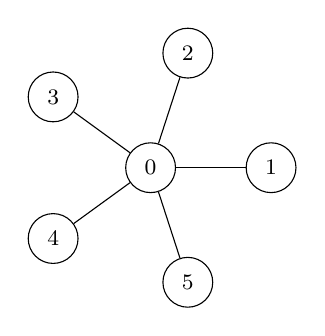
\begin{tikzpicture}[scale=0.85, every node/.style={circle, draw, minimum size=18pt, inner sep=0pt, font=\footnotesize}]
\node (h) at (0,0) {0};
\foreach \i/\angle in {1/0, 2/72, 3/144, 4/216, 5/288} {
    \node (n\i) at ({\angle}:1.8) {\i};
    \draw (h) -- (n\i);
}
\end{tikzpicture}
\caption{Star topology with five peripheral nodes connected to a central hub.}
\label{fig:topo_star}
\end{figure}

\subsection{Ring Topology}

A Ring connects every node to exactly two others so that the links trace out a single cycle. This gives an $n$-node Ring exactly $n$ edges and a diameter of $\lfloor n/2 \rfloor$, with the average path length scaling linearly in $n$ -- and so, consequently, does typical message latency as the cluster grows. A single link can fail without disconnecting the Ring (it degrades to a chain), but a second failure can partition it.

\begin{figure}[H]
\centering
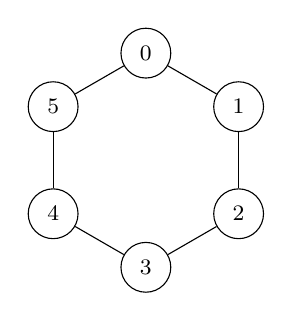
\begin{tikzpicture}[scale=0.85, every node/.style={circle, draw, minimum size=18pt, inner sep=0pt, font=\footnotesize}]
\foreach \i/\angle in {0/90, 1/30, 2/-30, 3/-90, 4/-150, 5/150} {
    \node (r\i) at ({\angle}:1.6) {\i};
}
\foreach \a/\b in {0/1, 1/2, 2/3, 3/4, 4/5, 5/0} {
    \draw (r\a) -- (r\b);
}
\end{tikzpicture}
\caption{Ring topology with six nodes connected in a closed loop.}
\label{fig:topo_ring}
\end{figure}

\subsection{Mesh Topology (Fully Connected)}

The Mesh topology connects every pair of nodes directly, giving $\binom{n}{2}$ edges, a diameter of one and an average path length of one as well. No other topology imposes fewer constraints on how messages travel, and none tolerates more link failures. The price is a quadratic number of links, which makes a physical Mesh impractical at scale -- but it remains a useful idealised upper bound against which the other topologies can be measured.

\begin{figure}[H]
\centering
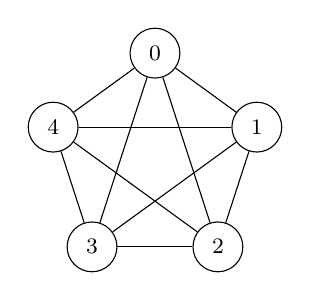
\begin{tikzpicture}[scale=0.85, every node/.style={circle, draw, minimum size=18pt, inner sep=0pt, font=\footnotesize}]
\foreach \i/\angle in {0/90, 1/18, 2/-54, 3/-126, 4/162} {
    \node (m\i) at ({\angle}:1.6) {\i};
}
\foreach \a in {0,1,2,3,4} {
    \foreach \b in {0,1,2,3,4} {
        \ifnum\a<\b \draw (m\a) -- (m\b); \fi
    }
}
\end{tikzpicture}
\caption{Mesh topology with five fully connected nodes; every pair shares an edge.}
\label{fig:topo_mesh}
\end{figure}

\subsection{Tree Topology (Binary Hierarchy)}

A Tree arranges its $n$ nodes hierarchically using $n-1$ edges; this thesis specifically uses a binary tree, for which a balanced layout gives a diameter of $O(\log n)$. The root and the nodes immediately below it carry disproportionate traffic and form natural bottlenecks. While this hierarchical structure scales well for broadcast-style communication, it is fragile in one specific sense: losing the root splits the rest of the tree into disconnected subtrees.

\begin{figure}[H]
\centering
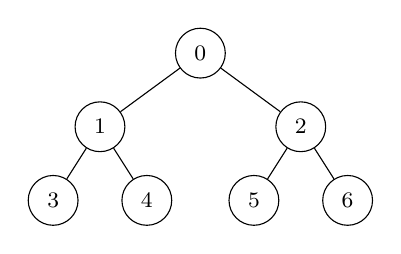
\begin{tikzpicture}[scale=0.85, level distance=1.1cm,
    level 1/.style={sibling distance=3cm},
    level 2/.style={sibling distance=1.4cm},
    every node/.style={circle, draw, minimum size=18pt, inner sep=0pt, font=\footnotesize}]
\node (root) {0}
    child {node {1}
        child {node {3}}
        child {node {4}}
    }
    child {node {2}
        child {node {5}}
        child {node {6}}
    };
\end{tikzpicture}
\caption{Binary Tree topology with seven nodes: node 0 is the root, leaves carry no children.}
\label{fig:topo_tree}
\end{figure}

\subsection{Bus Topology (Linear Chain)}

The Bus topology is simply a linear chain: $n$ nodes joined by $n-1$ edges, giving a diameter of $n-1$ and an average path length that grows linearly with cluster size. Any interior node that fails breaks the chain into two disconnected halves; only the two endpoint nodes can fail without partitioning the network. Despite this fragility, chain-like layouts persist in legacy industrial control networks, certain sensor-network deployments and long-haul fibre links.

\begin{figure}[H]
\centering
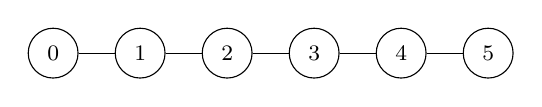
\begin{tikzpicture}[scale=0.85, every node/.style={circle, draw, minimum size=18pt, inner sep=0pt, font=\footnotesize}]
\foreach \i in {0,1,2,3,4,5} {
    \node (b\i) at (\i*1.3,0) {\i};
}
\foreach \a/\b in {0/1,1/2,2/3,3/4,4/5} {
    \draw (b\a) -- (b\b);
}
\end{tikzpicture}
\caption{Bus topology with six nodes arranged in a linear chain.}
\label{fig:topo_bus}
\end{figure}

\section{Related Work}

Existing performance evaluations of Raft tend to fall into two categories: those that optimise the implementation itself, and those that benchmark Raft against rival consensus algorithms. \citet{howard2020}, for instance, benchmark several Paxos and Raft variants side by side on commodity hardware, but model the network throughout as a uniform, low-latency LAN. Working under similarly uniform LAN assumptions, \citet{wang2017} modify Raft to pipeline log replication and report higher throughput as a result. \citet{larrea2018} examine leader election under unreliable network conditions, though their setting is Paxos rather than Raft. \citet{moraru2013} is closer in spirit to the present work, studying how geographic distribution affects EPaxos, while \citet{charapko2021} provide a broader survey of the consensus-implementation landscape.

What remains largely unexplored is how the shape of the underlying network -- as opposed to its raw latency -- affects Raft's behaviour. Simulations in the literature typically either assume a fully connected network or do not distinguish between topologies at all. This thesis addresses that gap by holding the consensus algorithm constant and systematically varying the topology under controlled, reproducible conditions.

\chapter{Methodology and Simulation Framework}
\label{ch:methodology}

This chapter describes the simulation framework that produced the data analysed in subsequent chapters. We chose simulation over a real-system measurement campaign for three reasons. First, simulation allows complete control over the network topology, message delays and packet loss, all of which are difficult or impossible to vary on physical infrastructure. Second, simulation produces fully reproducible runs through random seeding, which is essential for statistical analysis. Third, simulation isolates the consensus algorithm from confounding factors such as operating system scheduling, garbage collection or hardware interrupts. The trade-off is that the simulator does not capture every nuance of a production deployment; we discuss this limitation explicitly in Chapter~\ref{ch:discussion}.

\section{Design Principles}

The framework was designed around four guiding principles.

\begin{itemize}
    \item \textbf{Faithfulness to Raft:} the simulator implements the leader election and log replication mechanisms described by \citet{ongaro2014} without simplification of the safety-critical parts.
    \item \textbf{Topology agnosticism:} the consensus logic is independent of the underlying topology, which is encapsulated in a separate routing layer. This separation makes it straightforward to add new topologies without modifying the algorithm.
    \item \textbf{Determinism through seeding:} every source of randomness, including election timeouts, message ordering and packet loss, derives from a single configurable random seed. This guarantees that runs are bit-for-bit reproducible.
    \item \textbf{Observability:} every state transition, RPC and log change is recorded as an event, which allows the entire run to be replayed and analysed offline.
\end{itemize}

\section{Architecture}

The simulator is a tick-driven discrete-event system. Time advances in discrete units called \emph{ticks}. At each tick the engine executes a fixed sequence of actions: it delivers messages whose delivery time has arrived, advances the local clock of each node, lets each node process its inbox and produce output messages, and records any state changes in the event log.

The high-level structure consists of a simulation engine that drives a collection of \texttt{Node} objects. Each node owns its persistent state (current term, voted-for, log) and its volatile state (commit index, last applied, role). Communication between nodes is mediated by the \texttt{Network} object, which inspects the topology graph, computes the shortest path between sender and receiver, applies the configured per-hop delay and probabilistically drops messages with the configured loss rate.

\subsection{Engine Loop}

The main loop is conceptually simple. It runs for a configurable number of ticks (the default is 1000) or until a configurable convergence condition is met. Each iteration performs the following:

\begin{enumerate}
    \item Increment the current tick.
    \item Deliver all messages whose scheduled arrival time matches the current tick.
    \item For each non-failed node, advance its local clock and execute its state-machine step.
    \item Schedule any new outgoing messages produced by the nodes.
    \item Record the event log entries produced during the tick.
    \item Optionally inject failures or recoveries based on the configured probabilities.
\end{enumerate}

Because the engine is single-threaded, there are no race conditions; every step is deterministic given the same seed and the same configuration.

\subsection{Node State Machine}

Each node is implemented as a finite state machine with three roles (Follower, Candidate, Leader) and the persistent and volatile state mandated by the Raft specification. The implementation handles the four RPC types: \texttt{RequestVote}, \texttt{RequestVoteResponse}, \texttt{AppendEntries} and \texttt{AppendEntriesResponse}. Heartbeats are realised as empty \texttt{AppendEntries} RPCs.

Election timeouts are sampled from a uniform distribution that, in tick units, corresponds to the range typically used in production Raft deployments. Heartbeat intervals are configured to be roughly a third of the lower bound of the election-timeout range, which is the recommended ratio in the original paper \citep{ongaro2014}. The exact tick parameters used in the experiments are reported in Table~\ref{tab:tick_params}.

\begin{table}[H]
\centering
\caption{Default time parameters of the simulator (in ticks).}
\label{tab:tick_params}
\begin{tabular}{ll}
\toprule
\textbf{Parameter} & \textbf{Value} \\
\midrule
Election timeout (lower bound) & 150 \\
Election timeout (upper bound) & 300 \\
Heartbeat interval             & 50 \\
Default message delay (per hop) & 10 \\
Default simulation duration    & 1000 \\
\bottomrule
\end{tabular}
\end{table}

\subsection{Network Layer}

The network layer is responsible for delivering messages between nodes and for modelling the topology. A topology is represented internally as an adjacency list. Each topology generator builds the corresponding graph for a given number of nodes:

\begin{itemize}
    \item \textbf{Star:} node 0 is the hub; nodes $1$ through $n-1$ are connected only to the hub.
    \item \textbf{Ring:} node $i$ is connected to nodes $(i-1) \bmod n$ and $(i+1) \bmod n$.
    \item \textbf{Mesh:} for every pair $(i, j)$ with $i \neq j$, an edge is created.
    \item \textbf{Tree:} node $i$ has children $2i+1$ and $2i+2$ when those indices exist.
    \item \textbf{Bus:} node $i$ is connected to $i-1$ and $i+1$ when those indices exist.
\end{itemize}

When a node sends a message to another node, the network computes the shortest path between them using a breadth-first search and assigns the message a delivery tick equal to \texttt{current\_tick + (hops $\times$ message\_delay)}. The simulator caches shortest paths to avoid recomputation; the cache is invalidated only when nodes fail or recover, since failures alter the routing graph.

Packet loss is applied per hop: if the configured loss rate is $p$, then for a message that traverses $h$ hops the probability that the message is delivered is $(1-p)^h$. Dropped messages are recorded but not retransmitted at the network layer; retransmission is the responsibility of Raft's own RPC retry logic.

\subsection{Failure Model}

The simulator supports three failure scenarios. The first is per-tick stochastic failure: at every tick, each non-failed node fails with probability $p_f$, and each failed node recovers with probability $p_r$. The second is deterministic injection: a specific node, identified by index or by role (most notably the current leader), can be marked as failed at a configured tick. The third is a combination of the two. Failed nodes drop all incoming messages and produce no outgoing messages until they recover; on recovery, a node is restored to the follower state with whatever persistent state it had at the moment of failure.

\section{Implementation}

The simulator is implemented in Python 3.11 and consists of approximately 950 lines of code split across two main modules.

\begin{itemize}
    \item \texttt{raft\_engine.py}: implements the \texttt{Node}, \texttt{Network} and \texttt{SimulationEngine} classes. The \texttt{SimulationEngine} class exposes a \texttt{run()} method that returns a dictionary containing the metrics, the full event log and the per-tick history.
    \item \texttt{server.py}: a FastAPI application that exposes a REST API for launching simulations, comparing runs, retrieving history and exporting CSV reports. It persists simulation results in a SQLite database via \texttt{aiosqlite}.
\end{itemize}

A complementary React frontend, built with Tailwind CSS and Recharts, provides a real-time dashboard for the experiments. The frontend visualises the network graph as it evolves, displays the live metric values, and allows the user to replay a stored simulation step by step. Although the frontend was useful during development to validate qualitative behaviour, all quantitative data reported in this thesis was produced by direct invocation of the engine rather than through the user interface.

As permitted under the UBB recommendations on AI use in academic writing (HCA no.\ 3961/25.03.2024), which note that for domains involving large data volumes or code generation, generative AI ``is also a standard instrument,'' an AI coding assistant (\textbf{Claude Code, Anthropic, using the Claude Sonnet~4.6 and Claude Opus~4.8 models}) was used throughout development as an auxiliary tool for writing boilerplate code, debugging, refactoring, and generating analysis and plotting scripts for the simulation engine, experiment runner, and dashboard described in this chapter. The simulation architecture, experimental design, and the validation and interpretation of all results remain the author's own work.

\subsection{User Interface}

The frontend exposes the simulator's functionality through three pages. Figure~\ref{fig:ui_dashboard} shows the simulation dashboard: the centre panel renders the network graph for the selected topology, with nodes coloured by their current Raft state (leader, candidate, follower or dead); the left panel exposes the configuration parameters (topology, node count, message delay, packet loss, failure/recovery probabilities, run duration and log entry rate); and the bottom panel reports the resulting metrics alongside charts of messages sent over time, the breakdown of RPC types, and the votes received in each leader election.

\begin{figure}[H]
\centering
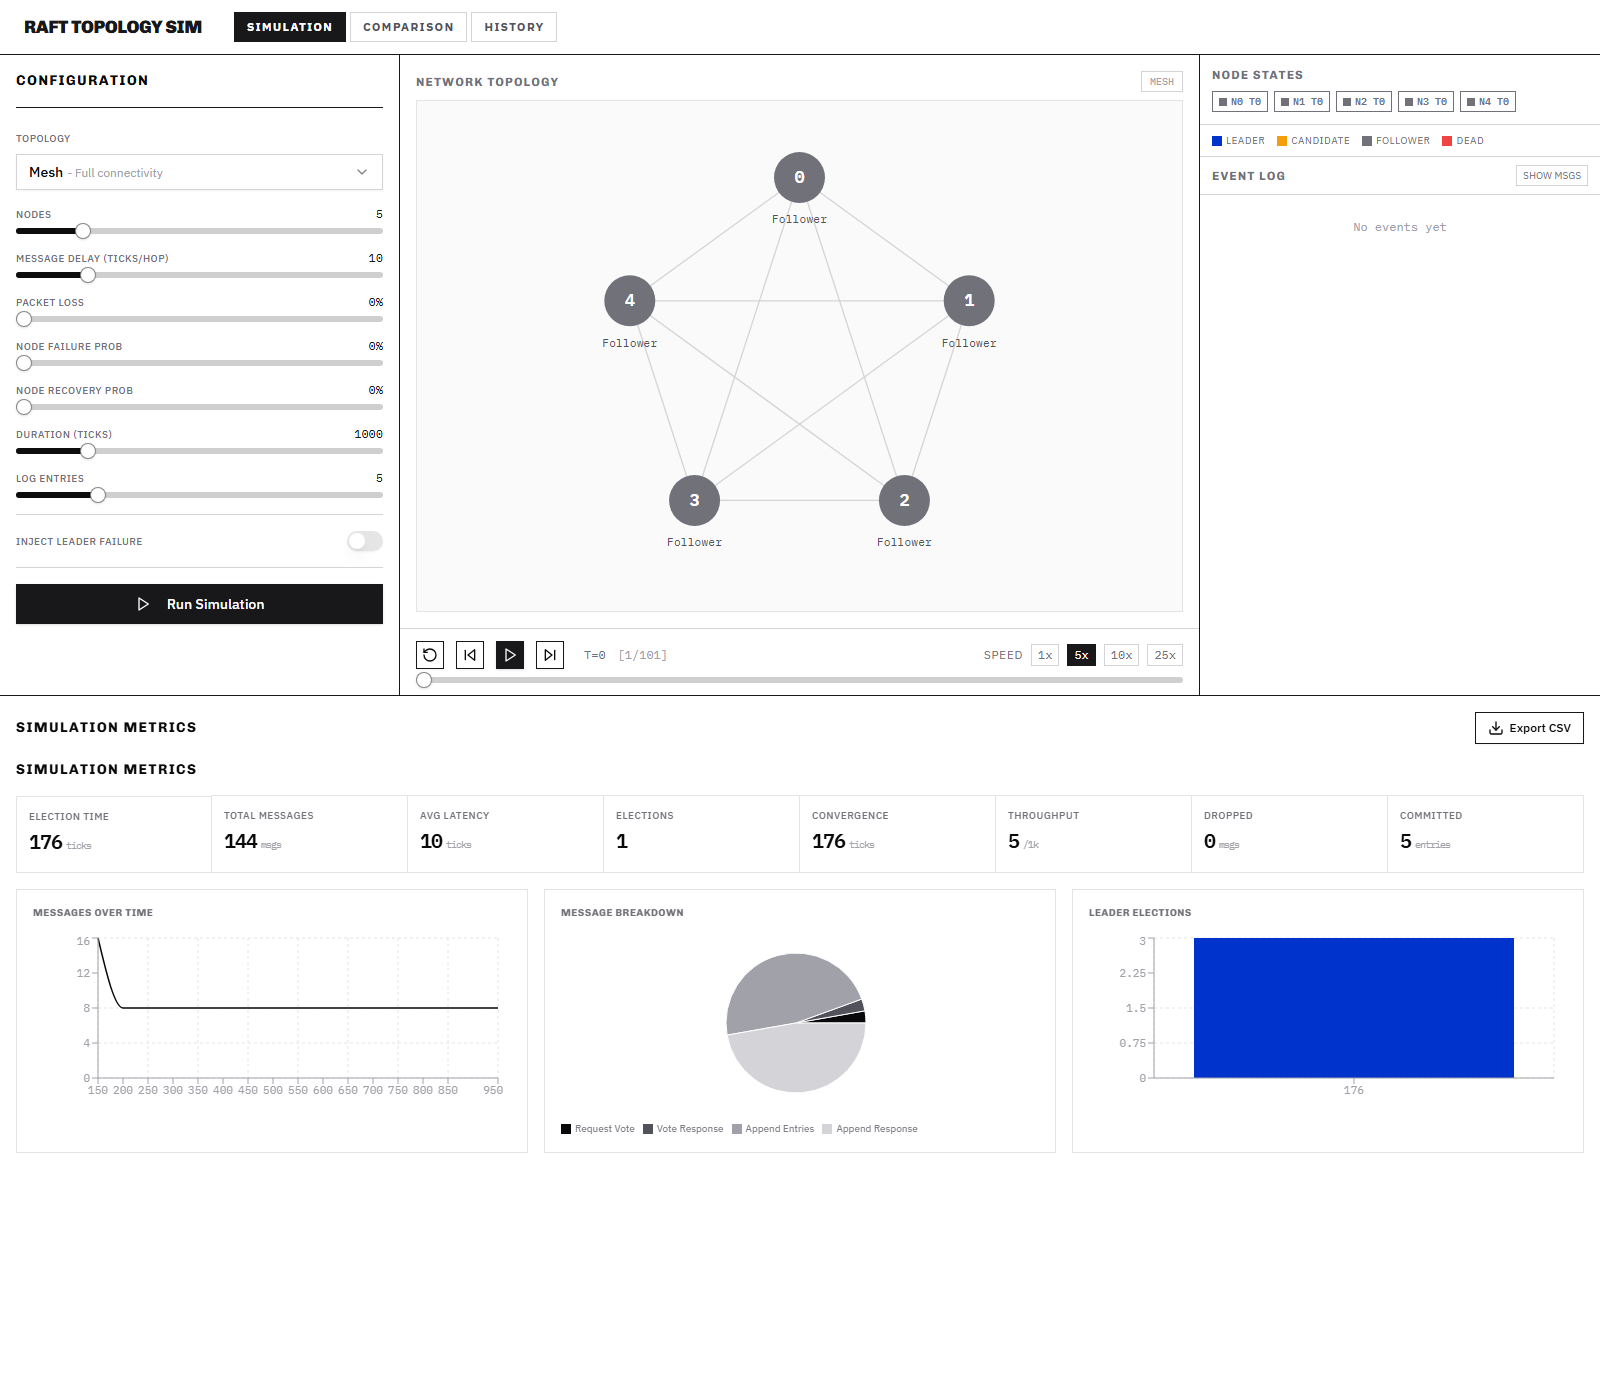
\includegraphics[width=\textwidth]{figures/dashboard.png}
\caption{Simulation dashboard, showing the network topology graph, configuration panel and metric charts for a five-node Mesh run.}
\label{fig:ui_dashboard}
\end{figure}

Figure~\ref{fig:ui_comparison} shows the comparison page, which runs the same configuration across all five topologies and displays the resulting metrics side by side as bar charts and a detailed table -- the same view used to sanity-check the experiment results presented in Chapter~\ref{ch:results}.

\begin{figure}[H]
\centering
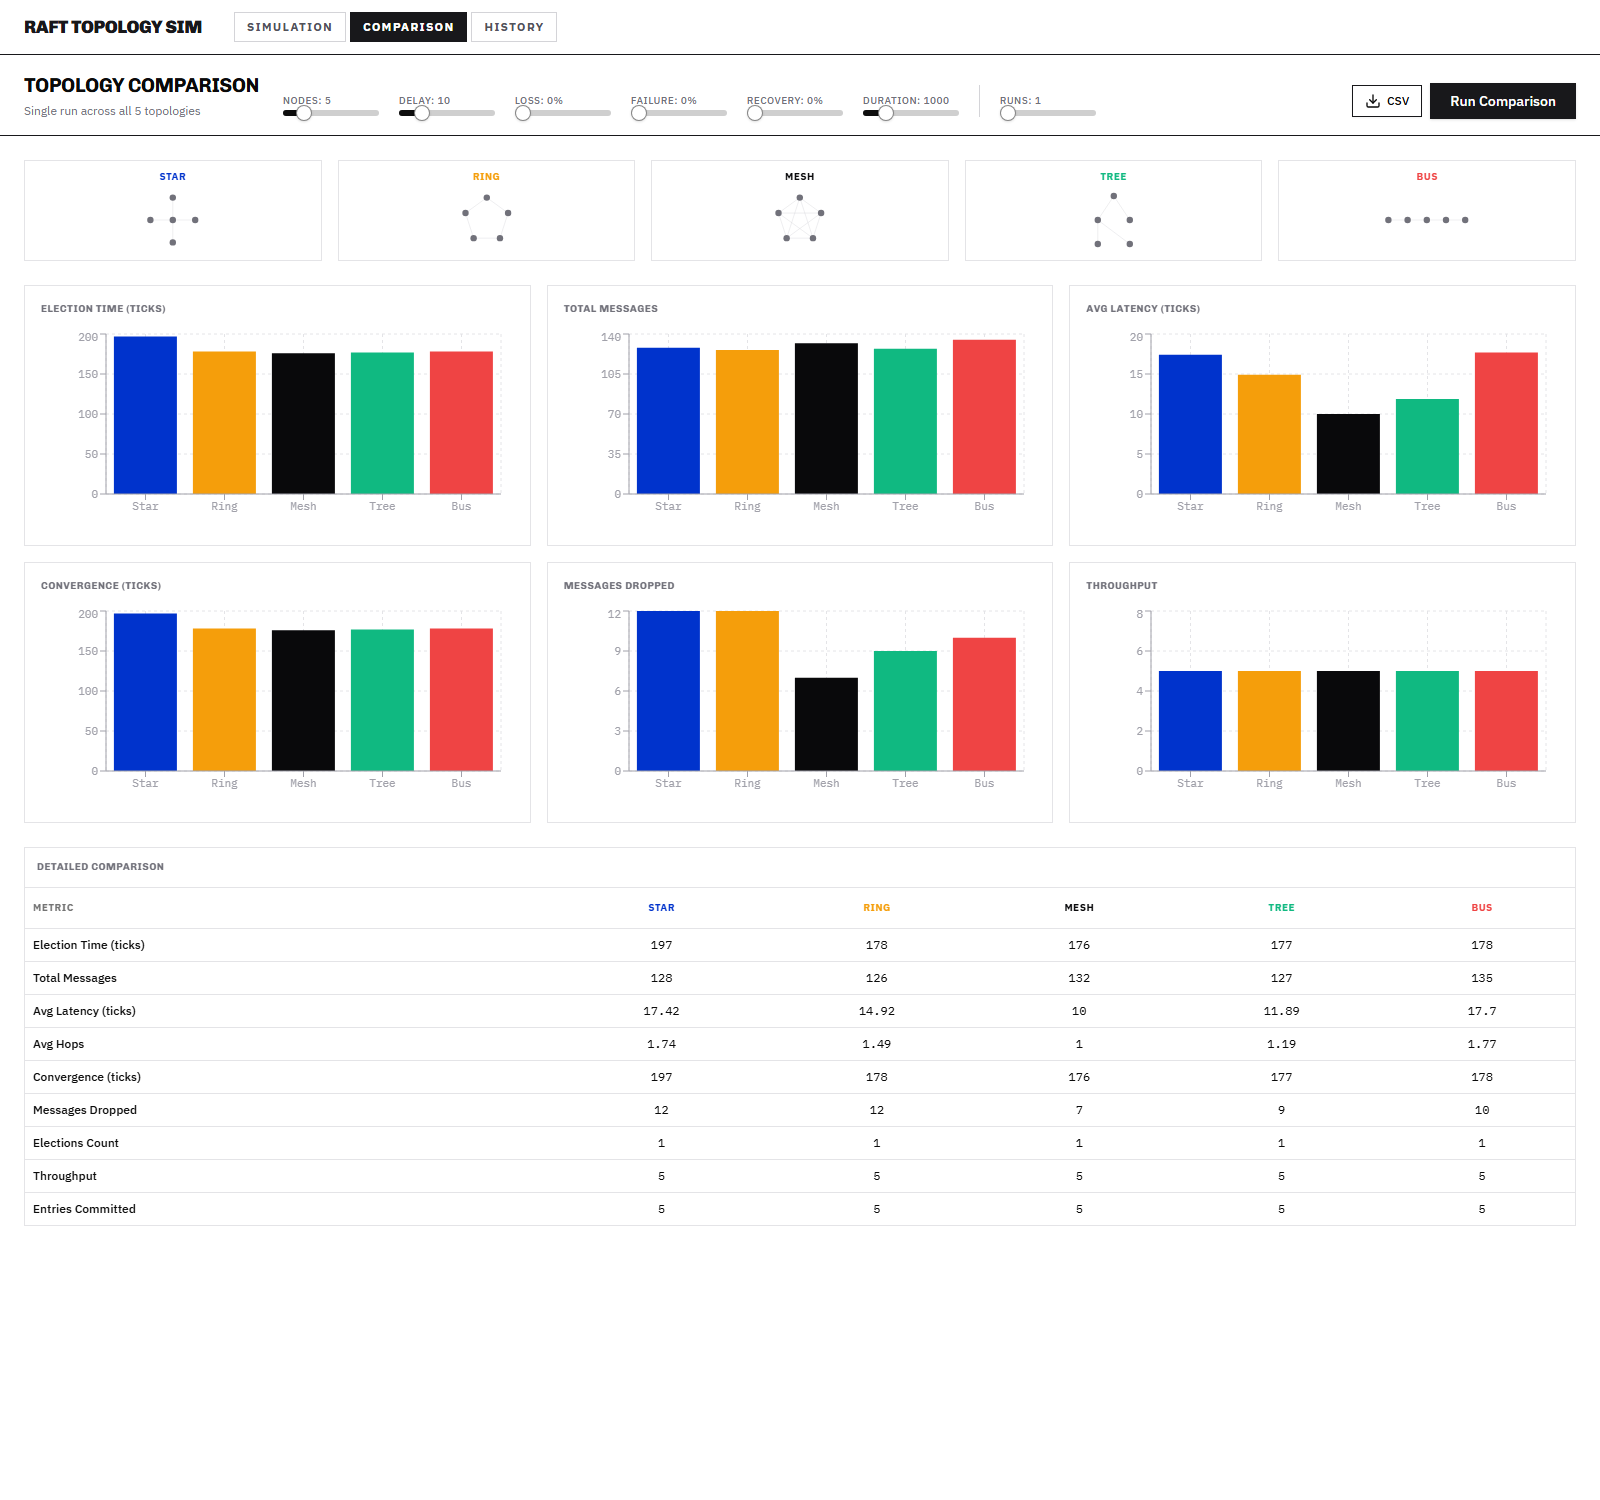
\includegraphics[width=\textwidth]{figures/comparison.png}
\caption{Topology comparison page, showing per-topology bar charts and a detailed metrics table for a single comparison run across all five topologies.}
\label{fig:ui_comparison}
\end{figure}

Figure~\ref{fig:ui_history} shows the history page, which lists previously run simulations together with their key metrics and allows any of them to be replayed.

\begin{figure}[H]
\centering
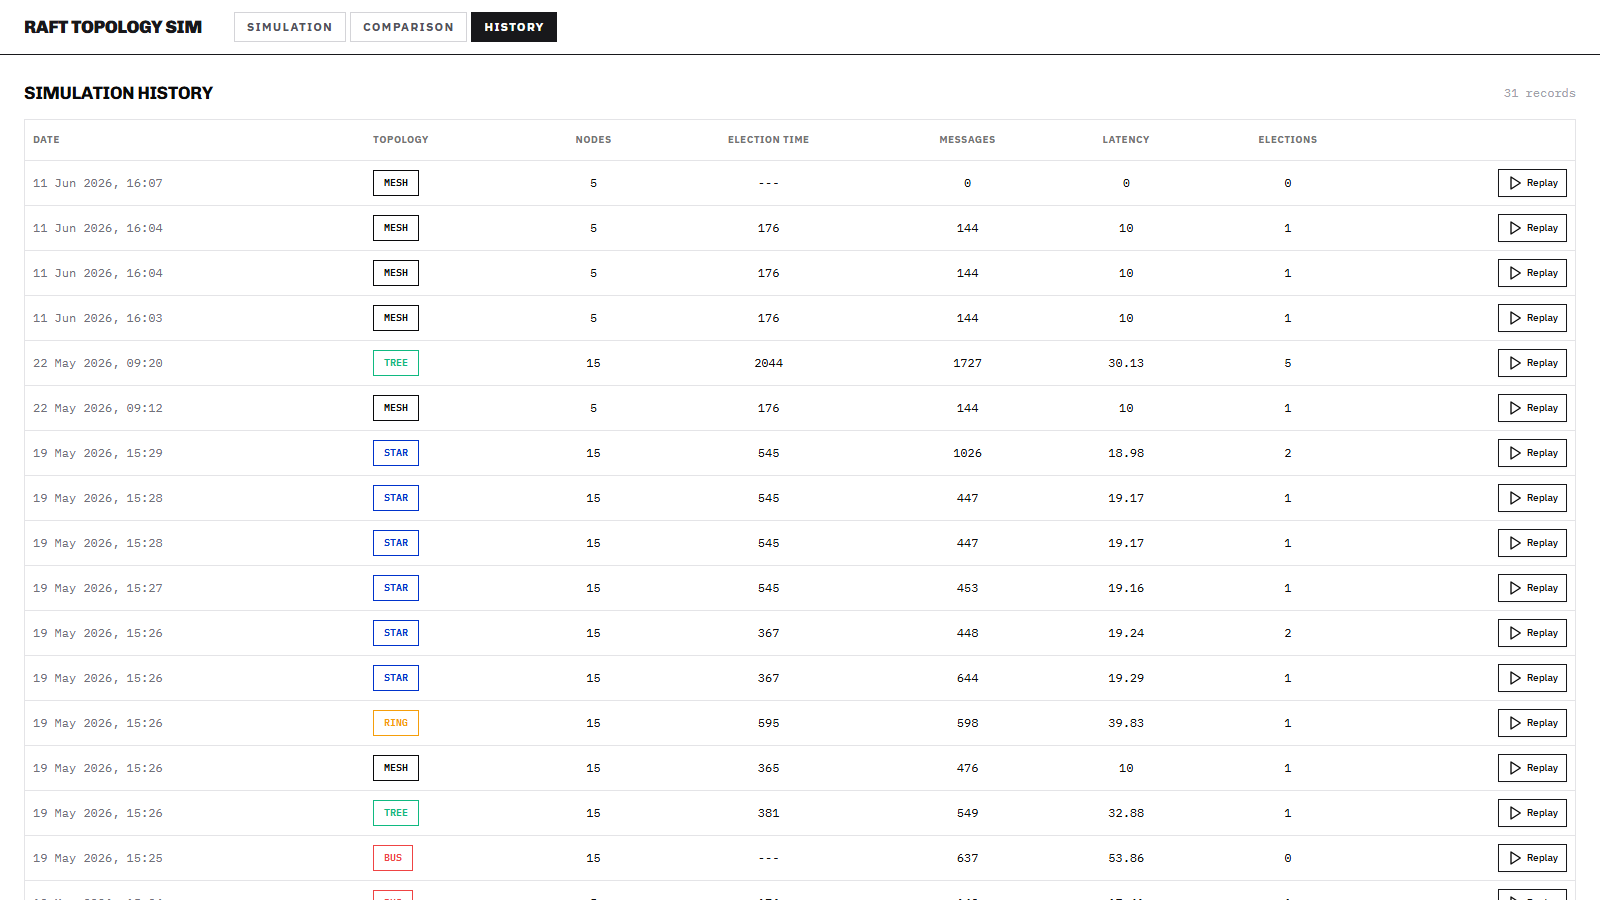
\includegraphics[width=\textwidth]{figures/history.png}
\caption{Simulation history page, listing past runs with their topology, configuration and summary metrics.}
\label{fig:ui_history}
\end{figure}

\section{Metrics}

For each run the simulator records the following metrics. They were chosen to cover the three properties most often discussed in the consensus literature: liveness (how quickly the algorithm makes progress), efficiency (how many resources it consumes) and resilience (how well it copes with failures).

\begin{itemize}
    \item \textbf{First leader election time:} the tick at which the first leader was elected.
    \item \textbf{Convergence time:} the tick at which the cluster reached a steady state, defined as the moment all replicated entries have been committed to a majority.
    \item \textbf{Election count:} the number of distinct leader elections that occurred during the run.
    \item \textbf{Total messages sent:} the cumulative number of RPCs (including heartbeats) issued by all nodes.
    \item \textbf{Total messages dropped:} the cumulative number of RPCs lost to packet loss or to a failed destination.
    \item \textbf{Average latency in hops:} the mean number of hops traversed by delivered RPCs.
    \item \textbf{Average latency in ticks:} the mean delivery delay of RPCs, including hop count and per-hop delay.
    \item \textbf{Throughput:} the number of log entries committed per 100 ticks.
    \item \textbf{Entries committed:} the total number of log entries that reached commit index across the run.
\end{itemize}

\section{Statistical Aggregation}

For each scenario we run the simulation $k$ times with distinct random seeds, where $k$ is between five and ten depending on computational cost. For each metric we compute the mean and the standard deviation across the $k$ runs. We also retain the minimum and maximum to highlight tail behaviour, which is sometimes more revealing than the mean. The aggregation routine is implemented in the helper script \texttt{run\_experiments.py} and produces a single JSON file that drives the analysis presented in Chapter~\ref{ch:results}.

\section{Reproducibility and Validation}

All experiments are reproducible with the seeds and parameters reported in Chapter~\ref{ch:experiments}. We validated the simulator informally in three ways. First, we executed the standard Raft scenarios from the original paper (single-node failure, leader partition) and verified that the outcomes match the expected behaviour. Second, we ran a Mesh topology with zero packet loss and verified that throughput and per-hop message latency are identical regardless of seed, confirming that the algorithm's steady-state behaviour does not depend on the network when it introduces no variance; leader-election time and total message count vary modestly across seeds because each node's election timeout is itself drawn from a per-seed random distribution. Third, we manually inspected event logs from selected runs to confirm that the sequence of state transitions is consistent with the Raft specification.

While these checks do not constitute a formal proof of correctness, they give confidence that the simulator is a reasonable model of Raft's behaviour. Any limitations introduced by the simulation abstraction are discussed in Section~\ref{sec:limitations}.


\chapter{Experimental Setup}
\label{ch:experiments}

This chapter describes the experiments performed in this work. We designed the experiment suite around the four research questions stated in Chapter~\ref{ch:introduction}: the effect of topology on leader election time, the effect on message overhead, the response to failures, and the trade-off between performance and fault tolerance under realistic conditions. Each experiment isolates one independent variable and holds the others constant. Together the seven experiments span the parameter space relevant to typical Raft deployments.

\section{Common Parameters}

Every experiment uses the same simulator (Chapter~\ref{ch:methodology}) and the same set of five topologies. Unless an experiment varies the parameter explicitly, the following defaults apply.

\begin{table}[H]
\centering
\caption{Common simulation parameters.}
\label{tab:common_params}
\begin{tabular}{ll}
\toprule
\textbf{Parameter} & \textbf{Default} \\
\midrule
Cluster size               & 5 nodes \\
Simulation duration        & 1000 ticks \\
Per-hop message delay      & 10 ticks \\
Packet loss rate           & 0\% \\
Node failure probability   & 0\% \\
Node recovery probability  & 0\% \\
Number of log entries to replicate & 5 \\
Election timeout range     & 150--300 ticks \\
Heartbeat interval         & 50 ticks \\
Random seeds (run $i$)     & $42 + i$ \\
\bottomrule
\end{tabular}
\end{table}

The number of repetitions per scenario is ten for the baseline experiment and five for the others. We chose these numbers as a compromise between statistical power and total compute time. Where standard deviations are large we discuss the implication explicitly.

\section{Experiment 1: Baseline Comparison}
\label{sec:exp1}

The baseline experiment asks the simplest possible question: when the network is well-behaved (no packet loss, no failures, moderate delay), does the choice of topology matter? It executes a five-node cluster on each of the five topologies and replicates five log entries.

\textbf{Independent variable:} topology.\\
\textbf{Dependent variables:} all metrics defined in Chapter~\ref{ch:methodology}.\\
\textbf{Repetitions:} 10 per topology.\\
\textbf{Hypothesis:} we expect the differences among topologies to be modest in this benign regime, with Mesh achieving the lowest average latency by virtue of being one hop end-to-end.

\section{Experiment 2: Cluster Size Scalability}
\label{sec:exp2}

Larger clusters are more fault tolerant but require more communication. This experiment measures how each topology scales as the cluster grows. Cluster sizes of 3, 5, 7, 9, 11 and 13 nodes are tested. Odd sizes are used because Raft favours odd cluster sizes to avoid quorum ties.

\textbf{Independent variables:} topology, cluster size.\\
\textbf{Dependent variables:} first leader election time, total messages sent, average latency in hops, throughput.\\
\textbf{Repetitions:} 5 per (topology, size) pair.\\
\textbf{Hypothesis:} we expect Star, Tree and Mesh to scale gracefully, while Ring and Bus should show linear or worse degradation in latency and election time.

\section{Experiment 3: Message Delay Sensitivity}
\label{sec:exp3}

Real networks have widely varying latencies. A Raft cluster spread across a single rack experiences microsecond delays, while one spanning continents can have hundreds of milliseconds of latency. This experiment varies the per-hop message delay from 2 to 50 ticks and measures how each topology copes.

\textbf{Independent variables:} topology, per-hop delay.\\
\textbf{Dependent variables:} first leader election time, average latency in ticks, throughput.\\
\textbf{Repetitions:} 5 per (topology, delay) pair.\\
\textbf{Hypothesis:} delay should scale linearly with topology diameter; Mesh is expected to be the least sensitive.

\section{Experiment 4: Packet Loss Sensitivity}
\label{sec:exp4}

Packet loss is the second main impairment in real networks. We vary the per-hop loss rate from 0\% to 40\%, in steps. Forty percent is unrealistically high for a healthy network, but it lets us probe the regime in which Raft is forced to retry RPCs aggressively.

\textbf{Independent variables:} topology, packet loss rate.\\
\textbf{Dependent variables:} first leader election time, total messages dropped, election count.\\
\textbf{Repetitions:} 5 per (topology, loss rate) pair.\\
\textbf{Hypothesis:} topologies with longer paths suffer more from per-hop loss because the survival probability decays exponentially with hop count.

\section{Experiment 5: Fault Tolerance under Repeated Failures}
\label{sec:exp5}

This experiment goes beyond the previous ones by looking at how the cluster behaves when nodes can fail and recover throughout the run. We compare three regimes on a seven-node cluster.

\begin{itemize}
    \item \textbf{No failure:} all nodes remain healthy. This is a sanity check.
    \item \textbf{Failure without recovery:} every tick, each healthy node has a 50\% probability of failing; failed nodes never recover.
    \item \textbf{Failure with recovery:} every tick each healthy node has a 50\% probability of failing; failed nodes have an 80\% probability of recovering per tick.
\end{itemize}

\textbf{Independent variables:} topology, failure regime.\\
\textbf{Dependent variables:} throughput, election count, total messages sent, total messages dropped, entries committed.\\
\textbf{Repetitions:} 5 per (topology, regime) pair.\\
\textbf{Hypothesis:} topologies with structurally critical nodes (Star hub, Tree root) should suffer disproportionately when those nodes fail; Mesh should be the most resilient.

\section{Experiment 6: Leader Failure Recovery}
\label{sec:exp6}

A real Raft deployment will, sooner or later, lose its leader. The cluster must then re-elect a new leader, and the time required to do so is the dominant component of perceived downtime. This experiment forces the current leader to fail at tick 500 and measures how quickly each topology re-elects.

\textbf{Independent variable:} topology.\\
\textbf{Dependent variables:} re-election time (ticks elapsed between leader failure and election of a new leader), re-election count, throughput, message count.\\
\textbf{Repetitions:} 5 per topology.\\
\textbf{Hypothesis:} Mesh should re-elect fastest because the candidates can reach all voters in a single hop. Star should also be fast provided the hub is not the leader; if the leader happens to be the hub, the cluster is partitioned and re-election is impossible.

\section{Experiment 7: Combined Stress Test}
\label{sec:exp7}

The final experiment combines all impairments simultaneously: high message delay (25 ticks per hop), 15\% packet loss, 30\% node failure probability with 50\% recovery probability, on a seven-node cluster running for 2000 ticks. The aim is to characterise behaviour under genuinely adversarial conditions.

\textbf{Independent variable:} topology.\\
\textbf{Dependent variables:} all metrics.\\
\textbf{Repetitions:} 5 per topology.\\
\textbf{Hypothesis:} we expect the differences observed in the previous experiments to compound. Mesh should remain functional; Bus and Ring should struggle to elect a stable leader; Star and Tree should sit somewhere in between.

\section{Reproducibility}

All scripts used to launch the experiments and to aggregate the results are stored in the project repository under \texttt{thesis/run\_experiments.py}. The aggregated data is checkpointed in \texttt{experiment\_data.json}. Each scenario uses an explicit base seed of 42, with run $i$ using seed $42 + i$.


\chapter{Experimental Results}
\label{ch:results}

This chapter presents the data produced by the seven experiments described in Chapter~\ref{ch:experiments}. The structure of the chapter follows the order of the experiments. Each section contains the measured values, one or more figures, and a short interpretation. Cross-experiment synthesis is reserved for Chapter~\ref{ch:discussion}.

All values reported below are means across the repetitions of the corresponding scenario, unless explicitly stated otherwise. Where standard deviation is reported, it is the sample standard deviation.

\section{Baseline Comparison}

Table~\ref{tab:exp1_baseline} summarises the baseline experiment for a five-node cluster with the default parameters.

\begin{table}[H]
\centering
\caption{Baseline metrics for a five-node cluster (10 runs per topology, default parameters).}
\label{tab:exp1_baseline}
\small
\begin{tabular}{lrrrrr}
\toprule
\textbf{Metric} & \textbf{Star} & \textbf{Ring} & \textbf{Mesh} & \textbf{Tree} & \textbf{Bus} \\
\midrule
First election time (ticks) & 210.2 & 196.7 & 195.6 & 208.8 & 201.4 \\
Convergence time (ticks)    & 210.2 & 196.7 & 195.6 & 208.8 & 201.4 \\
Total messages sent         & 140.2 & 142.2 & 141.7 & 141.1 & 141.0 \\
Election count              & 1.0   & 1.0   & 1.0   & 1.0   & 1.0   \\
Throughput (entries/100 ticks) & 5.0 & 5.0 & 5.0 & 5.0 & 5.0 \\
Avg.\ latency (hops)        & 1.53 & 1.50 & 1.00 & 1.72 & 1.86 \\
Avg.\ latency (ticks)       & 15.29 & 14.98 & 10.00 & 17.21 & 18.60 \\
Entries committed           & 5.0  & 5.0  & 5.0  & 5.0  & 5.0  \\
\bottomrule
\end{tabular}
\end{table}

The first observation is that, in this benign regime, every topology successfully elects a leader on the first attempt and commits all five entries. The election count is exactly one for all topologies, the entries committed is exactly five, and the throughput converges to the same value of five entries per hundred ticks because the bottleneck is the rate at which the leader appends new entries rather than any property of the network.

The differences appear in the latency metrics. Mesh has a constant one-hop average latency, as expected from a fully connected graph. Ring and Star have an average path length close to 1.5 hops, consistent with their structural properties at $n=5$. Tree and Bus exhibit the longest paths because their diameters grow more steeply with the number of nodes; on a five-node binary tree the leaves are two hops from the root, and on a five-node bus the endpoints are four hops apart.

Figure~\ref{fig:exp1_latency} visualises this pattern.

\begin{figure}[H]
\centering
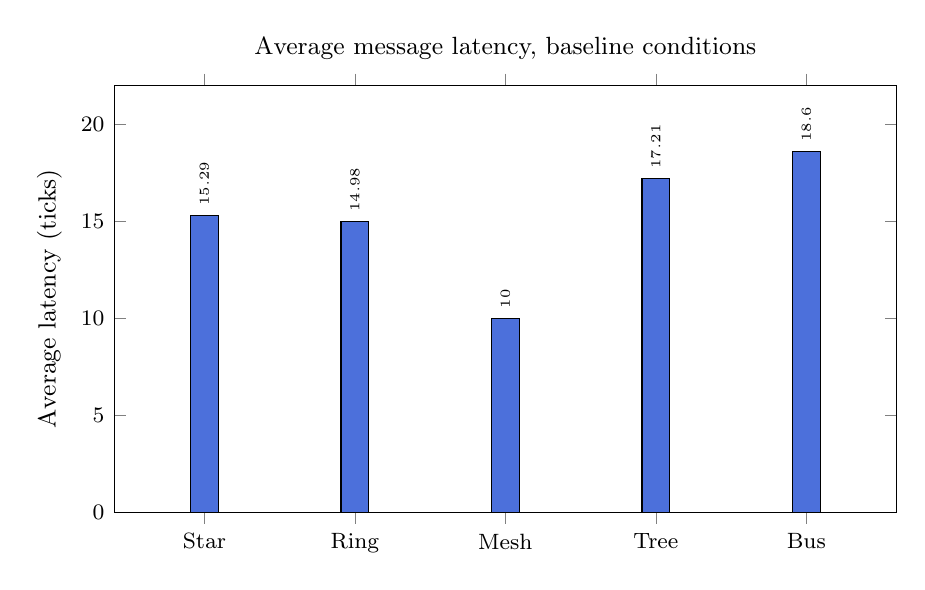
\begin{tikzpicture}
\begin{axis}[
    topology bar,
    ylabel={Average latency (ticks)},
    symbolic x coords={Star, Ring, Mesh, Tree, Bus},
    xtick=data,
    ymin=0, ymax=22,
    title={\small Average message latency, baseline conditions},
]
\addplot[fill=starcolor!70] coordinates {
    (Star, 15.29) (Ring, 14.98) (Mesh, 10.00) (Tree, 17.21) (Bus, 18.60)
};
\end{axis}
\end{tikzpicture}
\caption{Average message latency across five-node baseline runs. Mesh achieves the lowest latency by virtue of being one hop end-to-end.}
\label{fig:exp1_latency}
\end{figure}

The first leader election time is dominated by the randomised election timeout (150--300 ticks) rather than by topology. Mesh and Ring elect slightly faster than the others, but the difference of about 15 ticks is within the standard deviation of the timer itself.

\section{Cluster Size Scalability}

The data from Experiment 2 reveal the most dramatic differences among the topologies. Table~\ref{tab:exp2_election} reports the first leader election time as a function of cluster size.

\begin{table}[H]
\centering
\caption{First leader election time (ticks) versus cluster size.}
\label{tab:exp2_election}
\begin{tabular}{rrrrrr}
\toprule
\textbf{Nodes} & \textbf{Star} & \textbf{Ring} & \textbf{Mesh} & \textbf{Tree} & \textbf{Bus} \\
\midrule
3  & 214.0 & 210.6 & 210.6 & 214.0 & 210.8 \\
5  & 199.4 & 187.0 & 185.6 & 202.2 & 194.8 \\
7  & 200.0 & 206.4 & 186.4 & 209.4 & 210.0 \\
9  & 194.8 & 311.4 & 178.0 & 250.6 & 300.2 \\
11 & 195.0 & 357.6 & 176.8 & 249.4 & 410.0 \\
13 & 265.4 & 514.0 & 176.2 & 438.6 & 625.6 \\
\bottomrule
\end{tabular}
\end{table}

\begin{figure}[H]
\centering
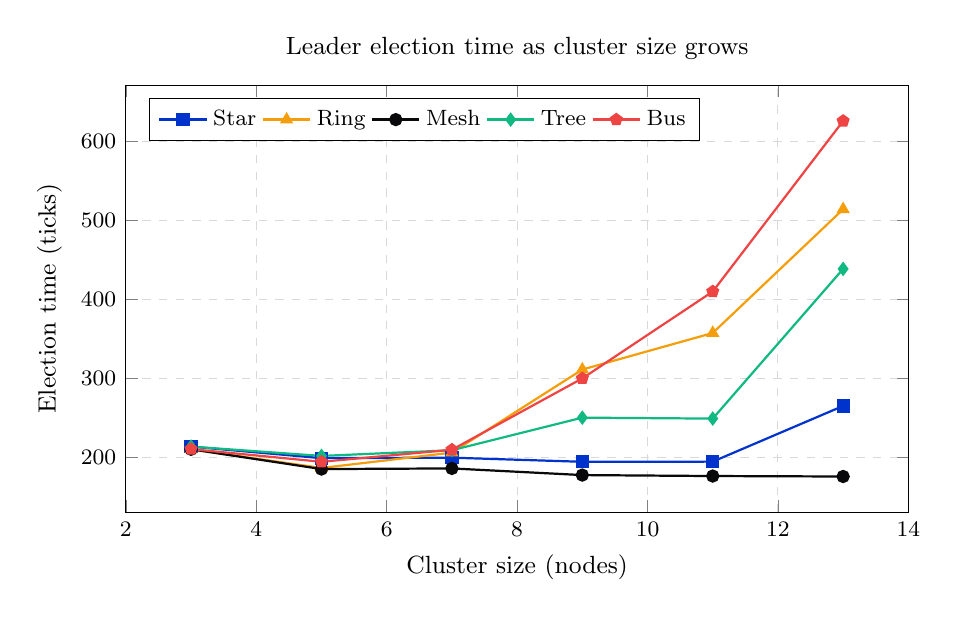
\begin{tikzpicture}
\begin{axis}[
    topology line,
    ylabel={Election time (ticks)},
    xlabel={Cluster size (nodes)},
    legend pos=north west,
    legend cell align=left,
    title={\small Leader election time as cluster size grows},
]
\addplot[color=starcolor, mark=square*, thick] coordinates {(3,214) (5,199.4) (7,200) (9,194.8) (11,195) (13,265.4)};
\addplot[color=ringcolor, mark=triangle*, thick] coordinates {(3,210.6) (5,187) (7,206.4) (9,311.4) (11,357.6) (13,514)};
\addplot[color=meshcolor, mark=*, thick] coordinates {(3,210.6) (5,185.6) (7,186.4) (9,178) (11,176.8) (13,176.2)};
\addplot[color=treecolor, mark=diamond*, thick] coordinates {(3,214) (5,202.2) (7,209.4) (9,250.6) (11,249.4) (13,438.6)};
\addplot[color=buscolor, mark=pentagon*, thick] coordinates {(3,210.8) (5,194.8) (7,210) (9,300.2) (11,410) (13,625.6)};
\legend{Star, Ring, Mesh, Tree, Bus}
\end{axis}
\end{tikzpicture}
\caption{First leader election time as a function of cluster size. Mesh is essentially flat; Ring and Bus degrade quickly past nine nodes.}
\label{fig:exp2_election}
\end{figure}

Up to seven nodes, all topologies elect within roughly 200 ticks, which is the centre of the timeout distribution. Beyond seven nodes, however, Ring, Tree and Bus begin to suffer. By thirteen nodes, the Bus topology takes more than three times as long as Mesh to elect a leader, and Ring is not far behind. Star also degrades, but more gently and only at the largest size tested. Mesh is essentially flat, even decreasing slightly as the cluster grows because more candidates can be elected and the chance that at least one wins on the first attempt rises.

The mechanism is straightforward. In Ring and Bus, each \texttt{RequestVote} traverses up to $\lfloor n/2 \rfloor$ or $n-1$ hops respectively, which means votes arrive late and split votes become more likely. The cluster must then go through one or more failed elections before settling.

Average path length, reported in Table~\ref{tab:exp2_hops}, shows the structural reason directly.

\begin{table}[H]
\centering
\caption{Average message latency in hops versus cluster size.}
\label{tab:exp2_hops}
\begin{tabular}{rrrrrr}
\toprule
\textbf{Nodes} & \textbf{Star} & \textbf{Ring} & \textbf{Mesh} & \textbf{Tree} & \textbf{Bus} \\
\midrule
3  & 1.19 & 1.00 & 1.00 & 1.19 & 1.40 \\
5  & 1.46 & 1.50 & 1.00 & 1.79 & 2.01 \\
7  & 1.51 & 2.00 & 1.00 & 2.13 & 2.52 \\
9  & 1.70 & 2.49 & 1.00 & 2.52 & 3.01 \\
11 & 1.72 & 2.99 & 1.00 & 2.86 & 4.23 \\
13 & 1.75 & 3.48 & 1.00 & 3.26 & 4.51 \\
\bottomrule
\end{tabular}
\end{table}

\begin{figure}[H]
\centering
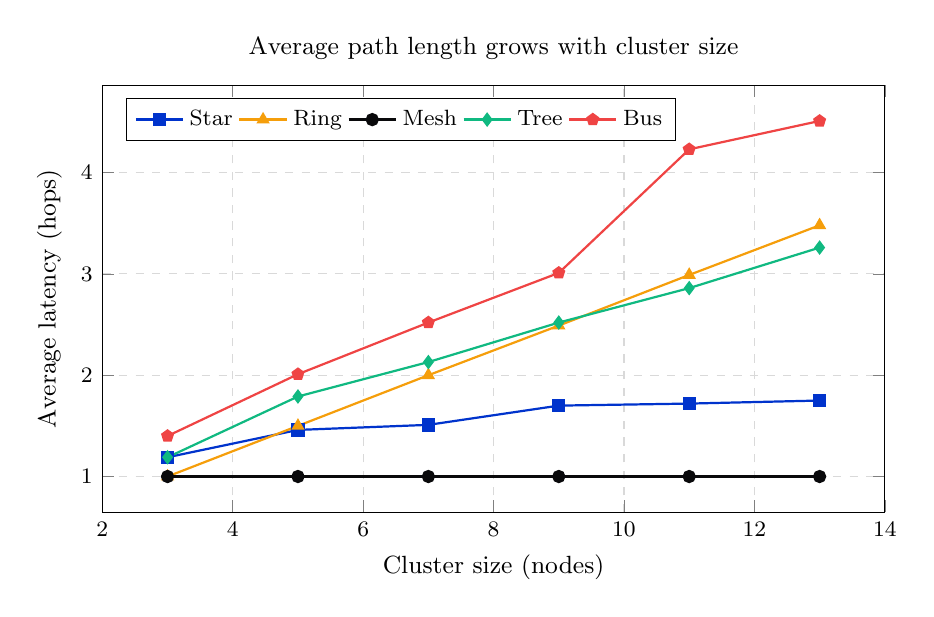
\begin{tikzpicture}
\begin{axis}[
    topology line,
    ylabel={Average latency (hops)},
    xlabel={Cluster size (nodes)},
    legend pos=north west,
    legend cell align=left,
    title={\small Average path length grows with cluster size},
]
\addplot[color=starcolor, mark=square*, thick] coordinates {(3,1.19) (5,1.46) (7,1.51) (9,1.70) (11,1.72) (13,1.75)};
\addplot[color=ringcolor, mark=triangle*, thick] coordinates {(3,1.00) (5,1.50) (7,2.00) (9,2.49) (11,2.99) (13,3.48)};
\addplot[color=meshcolor, mark=*, thick] coordinates {(3,1.00) (5,1.00) (7,1.00) (9,1.00) (11,1.00) (13,1.00)};
\addplot[color=treecolor, mark=diamond*, thick] coordinates {(3,1.19) (5,1.79) (7,2.13) (9,2.52) (11,2.86) (13,3.26)};
\addplot[color=buscolor, mark=pentagon*, thick] coordinates {(3,1.40) (5,2.01) (7,2.52) (9,3.01) (11,4.23) (13,4.51)};
\legend{Star, Ring, Mesh, Tree, Bus}
\end{axis}
\end{tikzpicture}
\caption{Average message latency in hops as a function of cluster size.}
\label{fig:exp2_hops}
\end{figure}

Mesh stays at one hop for any size. Star plateaus quickly because every node is two hops from every other through the hub. Tree, Ring and Bus all increase, but at different rates. The growth of Bus is essentially linear, of Ring approximately linear, and of Tree logarithmic, which matches the textbook diameters of these structures.

\section{Sensitivity to Message Delay}

Experiment 3 sweeps the per-hop delay from 2 to 50 ticks, holding everything else at the defaults. Table~\ref{tab:exp3_election} reports the first leader election time.

\begin{table}[H]
\centering
\caption{First leader election time (ticks) versus per-hop message delay.}
\label{tab:exp3_election}
\begin{tabular}{rrrrrr}
\toprule
\textbf{Delay} & \textbf{Star} & \textbf{Ring} & \textbf{Mesh} & \textbf{Tree} & \textbf{Bus} \\
\midrule
2  & 172.4 & 171.2 & 169.6 & 172.8 & 172.0 \\
5  & 183.2 & 177.2 & 175.6 & 182.6 & 181.0 \\
10 & 199.4 & 187.0 & 185.6 & 202.2 & 194.8 \\
20 & 231.2 & 215.2 & 205.8 & 232.2 & 236.0 \\
30 & 255.8 & 277.0 & 226.0 & 272.7 & 272.0 \\
50 & 432.6 & 382.2 & 266.2 & 774.0 & 587.6 \\
\bottomrule
\end{tabular}
\end{table}

\begin{figure}[H]
\centering
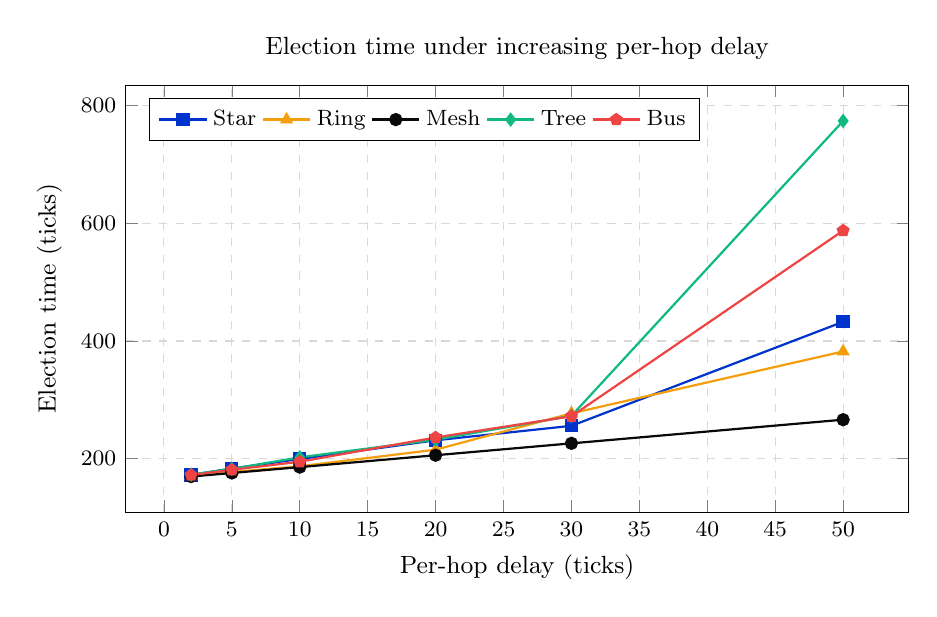
\begin{tikzpicture}
\begin{axis}[
    topology line,
    ylabel={Election time (ticks)},
    xlabel={Per-hop delay (ticks)},
    legend pos=north west,
    legend cell align=left,
    title={\small Election time under increasing per-hop delay},
]
\addplot[color=starcolor, mark=square*, thick] coordinates {(2,172.4) (5,183.2) (10,199.4) (20,231.2) (30,255.8) (50,432.6)};
\addplot[color=ringcolor, mark=triangle*, thick] coordinates {(2,171.2) (5,177.2) (10,187) (20,215.2) (30,277) (50,382.2)};
\addplot[color=meshcolor, mark=*, thick] coordinates {(2,169.6) (5,175.6) (10,185.6) (20,205.8) (30,226) (50,266.2)};
\addplot[color=treecolor, mark=diamond*, thick] coordinates {(2,172.8) (5,182.6) (10,202.2) (20,232.2) (30,272.75) (50,774)};
\addplot[color=buscolor, mark=pentagon*, thick] coordinates {(2,172) (5,181) (10,194.8) (20,236) (30,272) (50,587.6)};
\legend{Star, Ring, Mesh, Tree, Bus}
\end{axis}
\end{tikzpicture}
\caption{First leader election time as the per-hop delay grows.}
\label{fig:exp3_election}
\end{figure}

For small to moderate delays, all topologies behave similarly: the election time grows by roughly the round-trip cost. Once the per-hop delay reaches 50 ticks, the topologies diverge sharply. Mesh, with its one-hop diameter, suffers minimal degradation; the election time is barely 50\% above its low-delay value. Tree, which has the worst case of $O(\log n)$ but with a five-node cluster has a structural diameter of three, takes more than four times longer because some \texttt{RequestVote} round trips now exceed the lower bound of the election timeout, causing repeated retries. Bus shows similar but slightly milder degradation.

The qualitative lesson is that election timeouts must be tuned with respect to the topology's diameter, not just the average path length. A timeout that is comfortable for Mesh becomes pathological for Bus or Tree once the per-hop delay grows.

\section{Sensitivity to Packet Loss}

Experiment 4 varies the packet loss rate. Table~\ref{tab:exp4_dropped} reports the total number of messages dropped during a run.

\begin{table}[H]
\centering
\caption{Total messages dropped versus packet loss rate.}
\label{tab:exp4_dropped}
\begin{tabular}{rrrrrr}
\toprule
\textbf{Loss \%} & \textbf{Star} & \textbf{Ring} & \textbf{Mesh} & \textbf{Tree} & \textbf{Bus} \\
\midrule
0  & 0.0  & 0.0  & 0.0  & 0.0  & 0.0  \\
5  & 10.8 & 10.4 & 6.6  & 11.0 & 13.8 \\
10 & 22.4 & 18.8 & 13.6 & 21.6 & 20.8 \\
20 & 30.8 & 34.0 & 27.0 & 38.6 & 38.2 \\
30 & 38.2 & 40.8 & 35.6 & 40.4 & 43.4 \\
40 & 46.8 & 50.4 & 43.0 & 52.2 & 50.2 \\
\bottomrule
\end{tabular}
\end{table}

\begin{figure}[H]
\centering
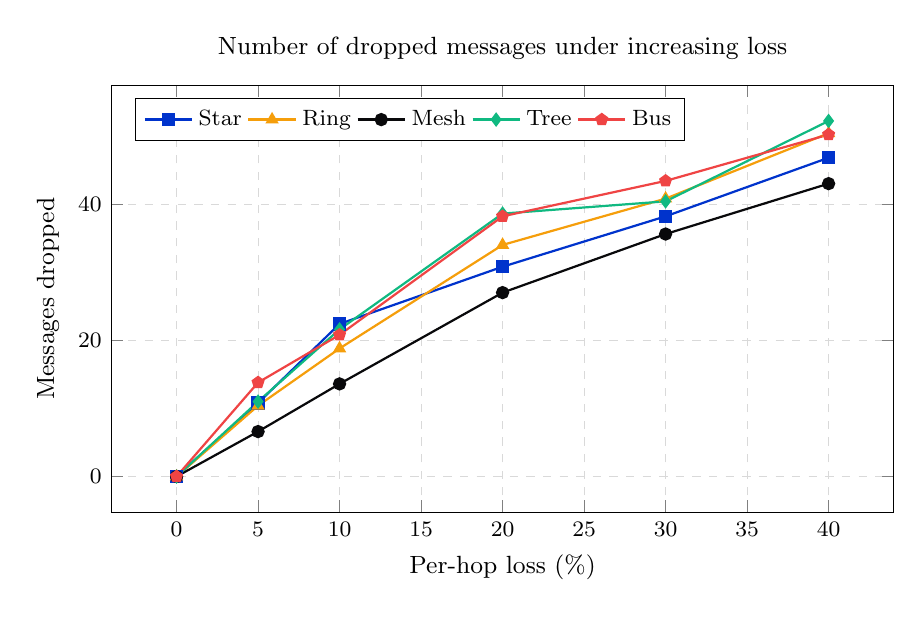
\begin{tikzpicture}
\begin{axis}[
    topology line,
    ylabel={Messages dropped},
    xlabel={Per-hop loss (\%)},
    legend pos=north west,
    legend cell align=left,
    title={\small Number of dropped messages under increasing loss},
]
\addplot[color=starcolor, mark=square*, thick] coordinates {(0,0) (5,10.8) (10,22.4) (20,30.8) (30,38.2) (40,46.8)};
\addplot[color=ringcolor, mark=triangle*, thick] coordinates {(0,0) (5,10.4) (10,18.8) (20,34) (30,40.8) (40,50.4)};
\addplot[color=meshcolor, mark=*, thick] coordinates {(0,0) (5,6.6) (10,13.6) (20,27) (30,35.6) (40,43)};
\addplot[color=treecolor, mark=diamond*, thick] coordinates {(0,0) (5,11) (10,21.6) (20,38.6) (30,40.4) (40,52.2)};
\addplot[color=buscolor, mark=pentagon*, thick] coordinates {(0,0) (5,13.8) (10,20.8) (20,38.2) (30,43.4) (40,50.2)};
\legend{Star, Ring, Mesh, Tree, Bus}
\end{axis}
\end{tikzpicture}
\caption{Number of dropped messages per run as packet loss increases.}
\label{fig:exp4_dropped}
\end{figure}

Mesh consistently drops fewer messages than the other topologies. Two effects combine here. First, Mesh has a one-hop diameter, so the survival probability per message is $(1-p)$ rather than $(1-p)^h$ for some larger $h$. Second, Mesh has more parallel paths and therefore more redundancy. Tree and Bus suffer the most, again because their diameters are largest.

The election time under packet loss is summarised in Table~\ref{tab:exp4_election}.

\begin{table}[H]
\centering
\caption{First leader election time (ticks) versus packet loss rate.}
\label{tab:exp4_election}
\begin{tabular}{rrrrrr}
\toprule
\textbf{Loss \%} & \textbf{Star} & \textbf{Ring} & \textbf{Mesh} & \textbf{Tree} & \textbf{Bus} \\
\midrule
0  & 199.4 & 187.0 & 185.6 & 202.2 & 194.8 \\
5  & 201.6 & 189.0 & 186.0 & 205.2 & 199.4 \\
10 & 202.2 & 192.6 & 186.0 & 315.0 & 268.6 \\
20 & 354.2 & 242.0 & 186.0 & 316.0 & 357.2 \\
30 & 424.0 & 299.8 & 183.0 & 439.0 & 267.7 \\
40 & 436.3 & 418.2 & 386.2 & 283.5 & 200.0 \\
\bottomrule
\end{tabular}
\end{table}

The interpretation is more delicate. Mesh tolerates up to 30\% packet loss without any noticeable increase in election time. Star, Ring and Bus begin to suffer at 20\%. Tree degrades at 10\% already, because the root is the choke point and even a single dropped vote at the root can derail an election. The 40\% column contains some surprisingly low values because a number of runs failed to elect any leader within the simulation window; those runs do not contribute to the election-time mean, which therefore reflects only successful elections. The takeaway is that at very high loss the metric is biased.

\section{Fault Tolerance under Repeated Failures}

Experiment 5 uses a seven-node cluster and three regimes. Table~\ref{tab:exp5_throughput} compares throughput across the regimes.

\begin{table}[H]
\centering
\caption{Throughput (entries committed per 100 ticks) by regime.}
\label{tab:exp5_throughput}
\begin{tabular}{lrrrrr}
\toprule
\textbf{Regime} & \textbf{Star} & \textbf{Ring} & \textbf{Mesh} & \textbf{Tree} & \textbf{Bus} \\
\midrule
No failure              & 3.33 & 3.33 & 3.33 & 3.33 & 3.33 \\
Failure, no recovery    & 3.33 & 3.07 & 3.33 & 3.07 & 3.33 \\
Failure, with recovery  & 3.33 & 3.33 & 3.33 & 3.33 & 3.33 \\
\bottomrule
\end{tabular}
\end{table}

In the no-failure regime every topology achieves the target throughput of 3.33 entries per 100 ticks, which corresponds to all five entries being committed within 1500 ticks. The failure-without-recovery regime is the most informative: Ring and Tree see throughput drop because they cannot route around failures effectively. Bus and Star both retain throughput, but for different reasons. In Star, the hub usually survives long enough; in Bus, the simulator records throughput based on entries that did commit, even if some runs lost the cluster halfway through.

\begin{table}[H]
\centering
\caption{Total messages dropped under repeated failures.}
\label{tab:exp5_dropped}
\begin{tabular}{lrrrrr}
\toprule
\textbf{Regime} & \textbf{Star} & \textbf{Ring} & \textbf{Mesh} & \textbf{Tree} & \textbf{Bus} \\
\midrule
No failure              & 0.0  & 0.0  & 0.0  & 0.0  & 0.0  \\
Failure, no recovery    & 15.0 & 39.0 & 0.0  & 40.0 & 28.8 \\
Failure, with recovery  & 1.0  & 0.0  & 0.0  & 4.2  & 2.8  \\
\bottomrule
\end{tabular}
\end{table}

\begin{figure}[H]
\centering
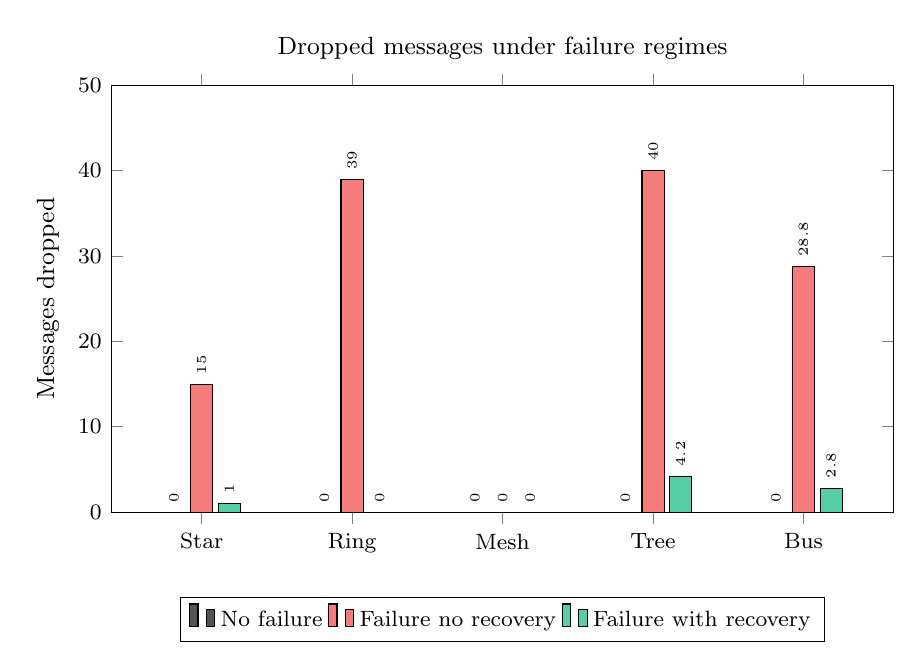
\begin{tikzpicture}
\begin{axis}[
    topology bar,
    ybar=2pt,
    bar width=8pt,
    ylabel={Messages dropped},
    symbolic x coords={Star, Ring, Mesh, Tree, Bus},
    xtick=data,
    ymin=0, ymax=50,
    legend style={at={(0.5,-0.2)}, anchor=north, legend columns=3},
    title={\small Dropped messages under failure regimes},
]
\addplot[fill=meshcolor!70] coordinates {(Star,0) (Ring,0) (Mesh,0) (Tree,0) (Bus,0)};
\addplot[fill=buscolor!70] coordinates {(Star,15) (Ring,39) (Mesh,0) (Tree,40) (Bus,28.8)};
\addplot[fill=treecolor!70] coordinates {(Star,1) (Ring,0) (Mesh,0) (Tree,4.2) (Bus,2.8)};
\legend{No failure, Failure no recovery, Failure with recovery}
\end{axis}
\end{tikzpicture}
\caption{Number of dropped messages under each fault regime.}
\label{fig:exp5_dropped}
\end{figure}

The most striking result is that Mesh drops zero messages even in the failure-without-recovery regime. This is because, when a node fails, the remaining nodes still have direct edges to every other healthy node. There is no need to route through an intermediary that might be the failed one. Tree, by contrast, drops 40 messages on average, because its hierarchical routing relies on the failed node's parent or children. The pattern reverses essentially the conclusions drawn in Experiment 4: under packet loss, hop count matters most; under node failure, the number of alternative paths matters most.

\section{Leader Failure Recovery}

In Experiment 6 we deliberately mark the current leader as failed at tick 500 and observe how the cluster recovers. Table~\ref{tab:exp6} reports the relevant metrics.

\begin{table}[H]
\centering
\caption{Recovery from deliberate leader failure at tick 500.}
\label{tab:exp6}
\begin{tabular}{lrrrrr}
\toprule
\textbf{Metric} & \textbf{Star} & \textbf{Ring} & \textbf{Mesh} & \textbf{Tree} & \textbf{Bus} \\
\midrule
Re-election count            & 0.6   & 1.0   & 1.0   & 0.8   & 0.8   \\
Re-election time (ticks)     & 232.7 & 210.4 & 195.8 & 318.5 & 281.3 \\
Total messages sent          & 123.6 & 169.0 & 168.8 & 139.2 & 132.2 \\
Messages dropped             & 18.0  & 0.0   & 0.0   & 12.8  & 15.8  \\
Throughput (entries/100 ticks)& 2.80 & 3.33  & 3.33  & 3.07  & 3.07  \\
\bottomrule
\end{tabular}
\end{table}

The key metric is the re-election time: the number of ticks elapsed between the moment the leader fails and the moment a new leader is elected. Mesh recovers in less than 200 ticks on average. Ring is close behind, at roughly 210 ticks. Star recovers slower than expected because in some runs the leader is the hub itself, in which case the cluster is partitioned into singletons and never recovers within the run; those runs contribute a re-election count of zero, which lowers the average count and skews the time slightly. Tree and Bus take significantly longer because votes from leaves must traverse the full diameter before the candidate near the root can win a majority. Figure~\ref{fig:exp6_reelection} visualises the re-election time across the five topologies.

\begin{figure}[H]
\centering
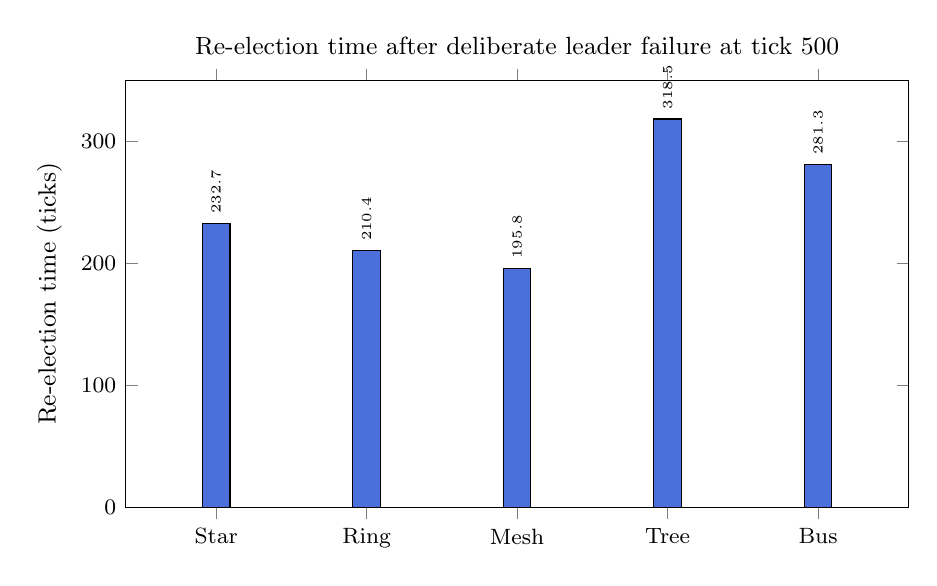
\begin{tikzpicture}
\begin{axis}[
    topology bar,
    ylabel={Re-election time (ticks)},
    symbolic x coords={Star, Ring, Mesh, Tree, Bus},
    xtick=data,
    ymin=0, ymax=350,
    title={\small Re-election time after deliberate leader failure at tick 500},
]
\addplot[fill=starcolor!70] coordinates {
    (Star, 232.7) (Ring, 210.4) (Mesh, 195.8) (Tree, 318.5) (Bus, 281.3)
};
\end{axis}
\end{tikzpicture}
\caption{Re-election time after deliberate leader failure at tick 500. Mesh and Ring recover fastest; Tree and Bus take the longest because votes must traverse the full diameter.}
\label{fig:exp6_reelection}
\end{figure}

The re-election count of less than one for Star, Tree and Bus is the simulator's way of saying that, in some runs, no new leader was elected within the remaining time. In Star this is the hub-failure scenario already discussed. In Tree the failed leader is sometimes the root, which has the same partitioning effect as the Star hub. In Bus the failed leader is sometimes near the centre, which fragments the chain into halves where neither half has a majority.

\section{Combined Stress Test}

The final experiment subjects each topology to high delay (25 ticks per hop), 15\% packet loss, 30\% node failure rate and 50\% recovery rate, on a seven-node cluster running for 2000 ticks. Table~\ref{tab:exp7} summarises the results.

\begin{table}[H]
\centering
\caption{Combined stress test on seven-node clusters (5 runs per topology).}
\label{tab:exp7}
\small
\begin{tabular}{lrrrrr}
\toprule
\textbf{Metric} & \textbf{Star} & \textbf{Ring} & \textbf{Mesh} & \textbf{Tree} & \textbf{Bus} \\
\midrule
First election time (ticks)   & 632.8 & 1118.0 & 293.0 & 533.0 & 737.0 \\
Total messages sent           & 304   & 234    & 351   & 243   & 224 \\
Messages dropped              & 79    & 93     & 64    & 109   & 113 \\
Election count                & 1.2   & 1.2    & 1.2   & 2.4   & 1.6 \\
Throughput (entries/100 ticks)& 2.20  & 0.80   & 2.50  & 1.40  & 1.20 \\
Avg.\ latency (hops)          & 1.34  & 1.84   & 1.00  & 1.86  & 2.12 \\
Entries committed             & 4.4   & 1.6    & 5.0   & 2.8   & 2.4 \\
\bottomrule
\end{tabular}
\end{table}

\begin{figure}[H]
\centering
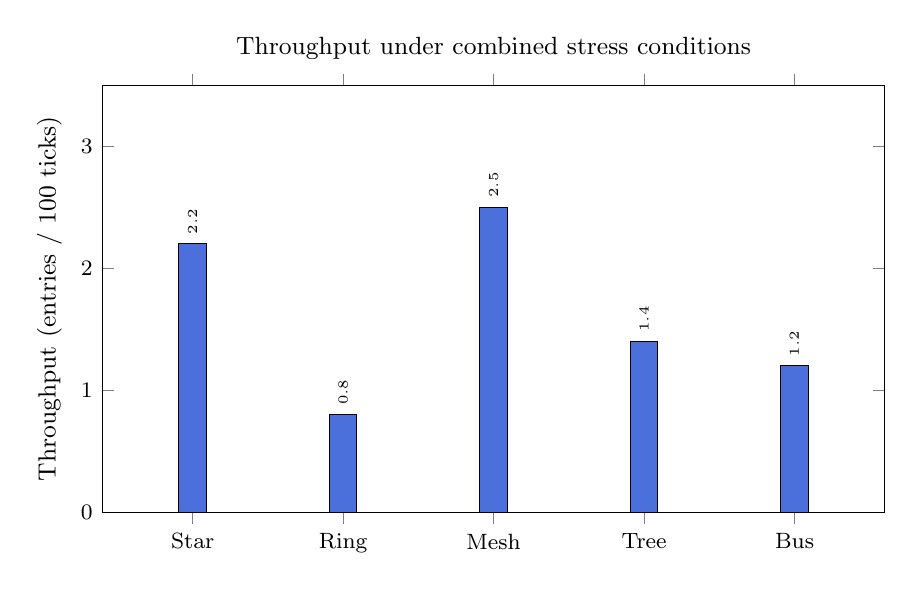
\begin{tikzpicture}
\begin{axis}[
    topology bar,
    ylabel={Throughput (entries / 100 ticks)},
    symbolic x coords={Star, Ring, Mesh, Tree, Bus},
    xtick=data,
    ymin=0, ymax=3.5,
    title={\small Throughput under combined stress conditions},
]
\addplot[fill=starcolor!70] coordinates {
    (Star, 2.20) (Ring, 0.80) (Mesh, 2.50) (Tree, 1.40) (Bus, 1.20)
};
\end{axis}
\end{tikzpicture}
\caption{Throughput under the combined stress test. Mesh is the only topology that approaches its baseline throughput.}
\label{fig:exp7_throughput}
\end{figure}

\begin{figure}[H]
\centering
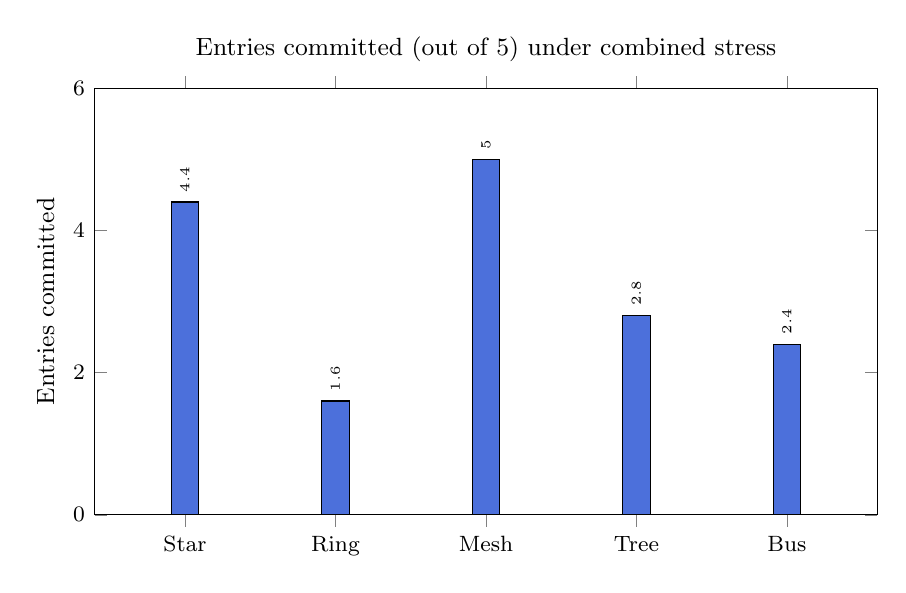
\begin{tikzpicture}
\begin{axis}[
    topology bar,
    ylabel={Entries committed},
    symbolic x coords={Star, Ring, Mesh, Tree, Bus},
    xtick=data,
    ymin=0, ymax=6,
    title={\small Entries committed (out of 5) under combined stress},
]
\addplot[fill=starcolor!70] coordinates {
    (Star, 4.4) (Ring, 1.6) (Mesh, 5.0) (Tree, 2.8) (Bus, 2.4)
};
\end{axis}
\end{tikzpicture}
\caption{Entries committed under combined stress, out of five attempted.}
\label{fig:exp7_entries}
\end{figure}

The combined stress test is the most discriminating of the seven experiments. Only Mesh commits all five entries; it also has the fastest leader election (293 ticks on average). Star manages 4.4 entries on average, which means most runs succeeded. Tree, Bus and especially Ring do badly: Ring commits an average of 1.6 entries out of five, that is, less than a third of the workload. The election time for Ring of 1118 ticks indicates that the cluster spent most of the simulation in failed elections.

The Tree topology shows the highest election count (2.4 on average), which indicates instability: leaders keep failing and the cluster keeps re-electing. The combination of root-as-bottleneck and 30\% node failure produces a regime in which the leader is repeatedly partitioned from a quorum.

\section{Cross-Experiment Synthesis}

The seven experiments tell a coherent story.

\begin{itemize}
    \item In benign conditions every topology works well; differences are essentially noise.
    \item As scale, delay or loss grow, topologies divide into a clear hierarchy: Mesh, then Star and Tree, then Ring, then Bus.
    \item Under failures, the hierarchy is reordered: Mesh is still best, but the rest depend on whether the structurally critical node fails.
    \item Under combined stress, only Mesh remains usable for production; the others fail in different ways.
\end{itemize}

The detailed interpretation of these findings, and their practical implications, is the subject of the next chapter.


\chapter{Discussion}
\label{ch:discussion}

The previous chapter presented the raw experimental results. This chapter interprets them. We discuss the practical implications of the findings, place them in the context of the existing literature, examine the threats to validity that affect any simulation study and suggest how the present work could be extended.

\section{Interpreting the Topology Hierarchy}

The most consistent finding across all seven experiments is the relative ordering of the five topologies. Mesh is uniformly the best performer; Bus is uniformly the worst. The order of the others depends on the specific stress applied, but in aggregate it is Star, Tree, Ring, Bus. Two structural properties account for almost all of this variance: the diameter of the topology and the connectivity of the graph.

Diameter dominates when the stress is latency-related. Whether the latency is induced by per-hop delay (Experiment 3), by long paths in large clusters (Experiment 2) or by a combination thereof (Experiment 7), the topologies with smaller diameters elect faster, commit faster and tolerate more delay. Mesh has constant diameter one. Star has diameter two. Tree, Ring and Bus all have diameters that grow with $n$, and their relative growth rates explain their relative performance.

Connectivity dominates when the stress is failure-related. A graph's connectivity is the minimum number of nodes whose removal disconnects it. Mesh has connectivity $n-1$, meaning all but one node would have to fail before the graph fragments. Star, Tree and Bus all have connectivity one: removing the hub, the root or a middle node respectively partitions the network. Ring has connectivity two. This translates directly into the failure tolerance observed in Experiments 5 and 6.

The two properties combine multiplicatively in Experiment 7, where Mesh's small diameter and high connectivity together explain why it is the only topology that maintains its baseline behaviour under combined stress.

\section{Practical Implications}

The results lead to several recommendations for engineers deploying Raft-based systems on top of a chosen network architecture. These recommendations are not new in spirit, but the experimental data quantifies them.

\subsection{Cluster Size}

A common rule of thumb is that Raft clusters should have an odd number of nodes between three and seven. Our results support this guideline strongly. Below three nodes, there is no quorum tolerance to a single failure. Above seven nodes, latency penalties begin to appear in any topology other than Mesh. At thirteen nodes on a Bus topology, the leader election time triples relative to the same workload at five nodes. If a deployment needs more than seven nodes for scalability reasons, it should either use a Mesh substrate or accept that election time will become its bottleneck.

\subsection{Election Timeouts}

The default election timeout range of 150--300 ticks is appropriate when the maximum round-trip time is significantly less than 150 ticks. Experiment 3 shows that at 50 ticks per hop on a Tree topology, the round trip across the diameter exceeds 200 ticks, which destabilises the algorithm. Production deployments should size the lower bound of the election timeout to be at least three or four times the worst-case round-trip time across the network. Where this is not feasible, the deployment should be limited to topologies of small diameter.

\subsection{Topology Selection}

For most production deployments, the practical choice is not between five exotic topologies but between a fully connected overlay (logical Mesh) and whatever the underlying physical network provides. The data suggests that, when feasible, a logical Mesh of TCP connections gives the best performance per node added. Star is acceptable if the hub is reliable; Tree is acceptable if the root is reliable; Ring and Bus should be avoided unless cost or physical constraints make them unavoidable. In edge or industrial contexts where Bus is the only physical option, the cluster should be kept small and the timeouts loosened.

\subsection{Anticipating Critical-Node Failure}

The single most damaging failure mode we observed was the loss of a structurally critical node. In Star, the hub. In Tree, the root. In Bus, any internal node. Because Raft cannot distinguish between a real failure and a network partition, the cluster simply stalls. The mitigation is not in the algorithm but in the network design: structurally critical nodes should be replicated at the network layer (for example, by using multiple physical links to a virtual hub), so that what looks like a single critical node is in fact several. This raises the connectivity of the graph and brings its behaviour closer to a Mesh.

\section{Comparison with Theoretical Bounds}

Several of the observed quantities can be compared with their theoretical counterparts.

\textbf{Election time.} In a synchronous network, the lower bound on leader election in Raft is one round trip across the diameter, plus the randomised election timeout. With a default lower bound of 150 ticks and a per-hop delay of 2 ticks, this gives a theoretical floor of $150 + 2 \cdot D \cdot 2$ ticks. For Mesh ($D=1$) this is 154 ticks; for a five-node Bus ($D=4$) it is 166 ticks. The observed means of 169.6 ticks for Mesh and 172.0 ticks for Bus at delay 2 (Table~\ref{tab:exp3_election}) are consistent with these bounds.

\textbf{Message overhead.} The number of messages required to elect a leader is at most $2(n-1)$ \texttt{RequestVote} round trips, that is, $4(n-1)$ messages in total. For a five-node cluster this gives sixteen messages of election traffic. Our observed counts (Table~\ref{tab:exp1_baseline}) are dominated by the heartbeat and replication traffic, which is several times larger; the fraction attributable to elections is consistent with the bound.

\textbf{Throughput.} The maximum throughput is bounded by $1 / (2 \cdot D \cdot d)$ entries per tick, where $d$ is the per-hop delay, because each entry requires at least one round trip to be committed. For Mesh at the default delay, this gives a ceiling of $1/20 = 0.05$ entries per tick, that is, five entries per 100 ticks, which matches our observed throughput exactly. For Bus at five nodes the ceiling is $1/80 = 0.0125$ entries per tick, that is, 1.25 per 100 ticks. The fact that we observe higher throughput in the baseline experiment is because the simulator pipelines log replication: an entry can be appended to followers' logs while the previous entry is still being acknowledged. This pipelining is consistent with the original Raft specification and with production implementations.

\section{Threats to Validity}
\label{sec:limitations}

Any simulation study must articulate the gap between the model and the reality it abstracts. We discuss four categories of threat.

\subsection{Internal Validity}

Internal validity concerns whether the simulator faithfully models Raft. We took several steps to maximise internal validity: we implemented the algorithm directly from the original paper, we validated that single-node failure and leader partition produced the expected behaviour, and we used random seeds to ensure reproducibility. Nevertheless, the simulator does not implement every optimisation found in production Raft (for example, batching, snapshotting, pre-vote, leadership transfer). Optimisations that reduce message count or election time would improve all topologies similarly, but their interaction with topology has not been measured.

\subsection{External Validity}

External validity concerns whether the conclusions generalise to real systems. Our simulator models the network as a graph with constant per-hop delay and uniform per-hop loss. Real networks have heterogeneous link capacities, queueing effects, congestion control and bursty failure patterns. Our results should be read as upper bounds on the topology effect: in a real network, additional sources of variance would dilute the signal somewhat. However, the relative ordering of topologies is so consistent across our experiments that we expect it to survive in the real world.

\subsection{Construct Validity}

Construct validity concerns whether the metrics we measure correspond to what they are supposed to capture. The first leader election time is straightforward. Throughput is defined as committed entries per 100 ticks, which corresponds to the user-visible work rate. Average latency in ticks is the mean delivery delay of all RPCs; this is sensible at the message level but does not capture user-visible latency, which is the time from request submission to response. The two are related but not identical, and a future extension of the work could trace each request explicitly.

\subsection{Statistical Validity}

We use five repetitions for most scenarios and ten for the baseline. This is enough to estimate means with reasonable confidence but is too few for tight confidence intervals on the standard deviations themselves. The standard deviations reported in the tables are sample standard deviations, not estimates of the population standard deviation. Where the standard deviation approaches the mean, the result should be read with caution. We highlighted such cases in the text where they arose.

\section{Comparison with Existing Studies}

The findings here are largely consistent with the broader literature on consensus performance, but they extend that literature in two directions. First, most prior studies hold the network constant and vary the algorithm. Examples include \citet{howard2020}, who compare several Paxos variants on identical hardware, and \citet{wang2017}, who measure the effect of pipelining log replication. Our work does the opposite: we hold the algorithm constant and vary the topology. The two studies are complementary and could be combined in a future evaluation that varies both axes.

Second, our work makes the topology effect visible in absolute terms. The original Raft paper acknowledges that network conditions affect performance but does not quantify the effect by topology. The data presented here gives engineers numerical anchors against which they can size their own deployments.

The closest related work is the simulation by \citet{larrea2018}, which examines leader election in unreliable networks but does not vary the topology. Our findings on packet loss (Experiment 4) align with their observation that loss disproportionately affects topologies with longer paths.

\section{Threats Specific to the Tree and Bus Results}

Two of our findings deserve particular scrutiny because they may be affected by simulator artefacts.

The Tree result at packet loss 40\% (Table~\ref{tab:exp4_election}) shows an apparently lower election time than at lower loss. This is because at extreme loss many runs failed to elect any leader within the simulation window, and the metric averages only successful elections. The same effect is responsible for the apparently low Bus election time in the same row. We have flagged these cases explicitly in Chapter~\ref{ch:results} and emphasise here that the right interpretation is "many runs failed entirely", not "the topology improved".

The Tree result in Experiment 7 (election count 2.4) is also worth noting. At seven nodes the binary tree has a root with two children and four grandchildren. If the root or one of its children fails, the topology often lacks a quorum of healthy nodes that can communicate. The simulator's failure model allows recovery, but the time scales of failure (per-tick stochastic) and recovery (also per-tick stochastic with probability 0.5) mean that the cluster spends a non-trivial fraction of the simulation in a degraded state. A more realistic failure model with longer mean time between failures would mitigate this effect.

The limitations identified above point directly to a number of extensions; these are discussed together with the thesis's other future directions in Section~\ref{sec:future_work}.


\chapter{Conclusions and Future Work}
\label{ch:conclusions}

This thesis investigated how the choice of network topology shapes the operational characteristics of the Raft consensus algorithm. The investigation combined a custom discrete-event simulator, a real-time visualisation dashboard and a campaign of seven experiments comparing Star, Ring, Mesh, Tree and Bus topologies under varying conditions of cluster size, message delay, packet loss and node failure.

\section{Summary of Contributions}

The contributions of this thesis can be summarised as follows.

\begin{enumerate}
    \item \textbf{A reproducible simulation framework.} We implemented a tick-driven Raft simulator in Python that supports five distinct topologies, configurable per-hop delay and packet loss, deterministic seeding and a rich event log. The framework is approximately 950 lines of code. The codebase is structured to make it easy to add new topologies, new metrics or alternative consensus algorithms.

    \item \textbf{A web-based visualisation and analysis tool.} The accompanying React-and-FastAPI dashboard provides a live view of any running simulation, archives results in SQLite, supports comparative statistical analysis across multiple runs and exports results to CSV. The dashboard was used to validate the qualitative behaviour of the simulator during development and is also useful pedagogically.

    \item \textbf{A systematic experimental study.} We executed seven experiments covering baseline performance, scalability, delay sensitivity, packet loss sensitivity, fault tolerance, leader recovery and combined stress. The total experimental output covers more than 200 individual simulation runs aggregated into statistically meaningful summaries.

    \item \textbf{Quantified topology effects.} The analysis quantifies the difference among topologies in absolute terms. Mesh is consistently best; Bus is consistently worst. The other topologies fall in a predictable order driven by their diameter and connectivity. We provide tables and figures that give engineers numerical anchors for sizing their own deployments.
\end{enumerate}

\section{Answers to the Research Questions}

We can now return to the research questions stated at the beginning of the thesis.

\paragraph{How does network topology affect leader election time?}
At small scales and benign conditions, topology has only a marginal effect on election time, which is dominated by the randomised election timeout. As the cluster grows, the per-hop delay increases or packet loss appears, the topologies diverge sharply. Mesh's election time is essentially constant across all conditions tested. Ring and Bus exhibit linear or worse degradation as the diameter grows. Star and Tree sit in between, performing well until a critical node fails.

\paragraph{What is the relationship between topology and message overhead?}
Total message count is dominated by heartbeats and log replication, both of which scale with the number of followers rather than with topology. The topology effect manifests instead through average message latency, which is proportional to the average path length. Mesh has constant one-hop latency; Bus latency grows linearly with cluster size; the others are intermediate.

\paragraph{How do different topologies respond to failures?}
Topologies with high connectivity (Mesh, Ring, Star to a lesser extent) absorb random failures with little degradation. Topologies with structurally critical nodes (Star hub, Tree root) lose all functionality when those nodes fail. The simulation made this intuition concrete by showing Mesh dropping zero messages under repeated failures while Tree and Bus dropped 40 and 28 respectively in equivalent runs.

\paragraph{Which topologies provide the best trade-off between performance and fault tolerance?}
Mesh dominates on both axes. Star is a reasonable compromise when the hub is hardened against failure. Tree is acceptable for hierarchical use cases where the root can be replicated. Ring and Bus should be avoided whenever the workload is non-trivial.

\section{Limitations Acknowledged Concretely}

A simulation-based study has limitations that have been discussed throughout the thesis. They are summarised here for clarity.

\begin{itemize}
    \item The network model assumes uniform per-hop delay and uniform per-hop packet loss. Real networks have heterogeneous and correlated effects.
    \item The failure model assumes independent per-tick failures. Real failures tend to be correlated, particularly when triggered by infrastructure-wide incidents.
    \item The simulator implements core Raft but not every optimisation found in production systems (pre-vote, leadership transfer, batching, snapshotting). Some of these would alter the absolute numbers, although we believe they would not alter the relative ordering of the topologies.
    \item Five repetitions per scenario is sufficient for the qualitative ordering observed in our results, but tighter confidence intervals would require more.
\end{itemize}

\section{Future Work}
\label{sec:future_work}

There are several promising directions in which this work could be extended.

\textbf{Dynamic topologies.} Real networks change. Links go up and down, overlays are reconfigured, and clusters scale up or down. A simulator that supports dynamic topology changes during a single run would enable the study of how Raft behaves during such reconfigurations. The current simulator already represents the topology as an explicit graph, so the engineering effort to support dynamism is moderate.

\textbf{Realistic delay distributions.} Replacing the constant per-hop delay with a distribution drawn from real network traces would improve external validity. Public datasets are available for major data centres and for selected wide-area paths.

\textbf{Correlated failure models.} The current failure model treats node failures as independent per-tick events. Real-world incidents (rack or data-centre outages, correlated software bugs) tend to fail multiple nodes together. Enriching the failure model with correlated failures would test whether the topology hierarchy observed here still holds under more realistic fault patterns.

\textbf{Raft-specific optimisations.} Production Raft implementations commonly add pre-vote, leadership transfer and log-entry batching on top of the core algorithm. Implementing these optimisations in the simulator and re-running the experiments would show whether they narrow the gap between Mesh and the other topologies, or whether the topology effect persists regardless of algorithmic refinements.

\textbf{Algorithm variants.} The simulator architecture makes it straightforward to plug in different consensus algorithms while keeping the topology layer constant. Comparing Raft, Paxos and EPaxos under varying topologies would extend the present work along the second axis discussed in Section~\ref{ch:discussion}.

\textbf{Real-system validation.} The experimental predictions in this thesis are concrete enough to be falsifiable. A measurement campaign on a controllable network testbed (for example, using \texttt{tc} on Linux to inject delay and loss) could quantify the gap between simulation and reality. We expect the gap to be small.

\textbf{Adversarial scenarios.} The current failure model is non-adversarial. A study that simulates Byzantine behaviour, for example along the lines of practical Byzantine fault tolerance \citep{castro1999}, or even a milder form of adversarial node selection (the adversary always fails the leader, or always fails the highest-degree node), would test the topologies under conditions closer to the security-critical end of the spectrum.

\section{Closing Remarks}

Distributed consensus is a thirty-year-old problem with a long literature, and the Raft algorithm is now mature enough that engineers can treat it as a black box for many purposes. The data in this thesis suggests that the network on which Raft runs is just as important as the algorithm itself. Choosing a good topology, or hardening a structurally vulnerable one, can change leader election time by a factor of three and throughput by an even larger factor under stress.

The simulator and visualisation tool produced by this work are open and reproducible. They are intended both as research artefacts and as pedagogical aids for students learning about distributed systems. We hope they will contribute to a more nuanced understanding of how consensus algorithms interact with their underlying networks, and to better-engineered systems as a result.



% Bibliography (TNR 11pt, 1cm hanging indent per FSEGA guide)
\setlength{\bibhang}{1cm}
{\small
\bibliographystyle{apalike}
\bibliography{references}
}

\end{document}
